\documentclass[11pt]{article}

\usepackage[margin=1in]{geometry}
\usepackage{amsmath,amssymb,amsthm}
\usepackage{array}
\usepackage{booktabs}
\usepackage{caption}
\usepackage{xcolor}
\usepackage{graphicx}
\usepackage{microtype}
\usepackage{hyperref}

\graphicspath{{docs/figure_assets/submission_draft_python_figures/outputs/}{../figure_assets/submission_draft_python_figures/outputs/}{../../docs/figure_assets/submission_draft_python_figures/outputs/}}

\emergencystretch=2em

\newcommand{\hardwareclaimrequired}{\textit{Required for hardware claim}}
\newcommand{\softwarehil}{controlled simulation}
\newcommand{\finalLER}{\texttt{final\_ler\_mean}}
\newcommand{\methodname}{runtime-consistent affine calibration}
\newtheorem{proposition}{Proposition}

\title{Affine Runtime Calibration for Drift-Adaptive Gottesman--Kitaev--Preskill Decoding}
\author{Anonymous authors}
\date{}

\begin{document}
\maketitle

\begin{abstract}
Fault-tolerant quantum processors require classical correction layers that can
adapt to analog drift without placing unbounded computation on the feedback
path.  Approximate Gottesman--Kitaev--Preskill (GKP) error correction is a
natural setting for this problem because continuous modular syndromes must be
converted into displacement corrections, while finite-energy peaks, noisy
auxiliary measurements and calibration drift make a fixed correction surface
brittle.  We study runtime-consistent affine calibration, in which the
per-shot fast path is constrained to
\(\Delta_t = K_t s_t + b_t\) and a slower loop updates \((K_t,b_t)\) from recent
analog syndrome statistics.  This separates drift adaptation from the
latency-critical correction: neural, teacher-anchored or statistical estimators
may propose the next affine surface, but every shot is corrected by the same
deterministic matrix-vector rule.  In a predeclared four-scenario controlled
simulation, the teacher-anchored hybrid residual branch has the lowest mean
protocol-defined \finalLER{} in all tested drift scenarios, reducing
\finalLER{} relative to an unscented Kalman filter by \(1.8\)--\(2.9\%\)
(\(2.3\%\) on average).  Two 12-pair scenario checks, for
\texttt{static\_bias\_theta} and \texttt{linear\_ramp}, give positive
UKF-minus-hybrid lower bounds under both paired-\(t\) and bootstrap summaries.
Controlled nearest-syndrome, oracle-affine, wrapped-Gaussian, holdout-stress
and residual-boundary channel diagnostics show where the affine contract is
useful and where it remains narrower than finite-energy logical-channel
fidelity.  The fast path requires four multiplications, four additions and six
stored state scalars per shot, and Q4.20 software emulation changes no
residual-boundary crossing rates in the controlled sample set.  The evidence
supports an interface-level claim: within the tested controlled-simulation
setting, drift-adaptive GKP correction can be exposed through a small, logged
affine surface while preserving a deterministic correction path suitable for
fixed-point replay.  Board latency, resource use, power and source-vs-board
agreement are reserved for device validation.
\end{abstract}

\section{Introduction}

Quantum error correction is increasingly a real-time control problem as well
as a coding problem.  A useful decoder must interpret noisy measurements,
adapt to calibration drift and still return a correction within the timing
budget of the physical experiment.  Bosonic quantum error correction adds a
distinct opportunity and challenge: oscillator measurements are continuous, so
they carry analog reliability information, but the classical control stack must
decide which part of that information can be used immediately and which part
should update a slower calibration state.  The GKP code is a prominent example:
shift errors are inferred from modular quadrature syndromes and corrected by
displacement operations \cite{gkp2001,grimsmo2021}.  In an idealized setting,
the decoder can treat each measured syndrome as a local displacement estimate.
In a physical setting, approximate finite-energy GKP states, noisy auxiliary
measurements and hardware calibration drift alter the distribution seen by the
decoder over time.

The resulting bottleneck is not only statistical accuracy, but the interface
between estimation and real-time control.  A drift-aware decoder should exploit
recent analog syndrome information, yet a decoder intended for a hardware
control stack must expose a small, testable and latency-bounded correction
surface.  End-to-end neural decoding can be expressive, but it obscures
worst-case timing, fixed-point degradation and rollback behaviour.  A fixed
affine correction law has the opposite profile: it is fast
and interpretable, but it cannot by itself follow bias, variance or
orientation drift in the effective GKP noise state.

We separate these two responsibilities.  The fast loop is limited
to a two-quadrature affine rule,
\begin{equation}
    \Delta_t = K_t s_t + b_t ,
    \label{eq:fastpath}
\end{equation}
where \(s_t\) is the measured syndrome and \((K_t,b_t)\) are the active
runtime parameters.  The slow loop updates these parameters from a recent
syndrome histogram, teacher estimate or statistical calibration rule.  The
learned component is therefore not the per-shot decoder; it is one possible
slow-loop module for recalibrating a low-dimensional physical displacement
rule.  Different estimators can be compared only after they commit the same
type of \((K,b)\) parameters to the deterministic fast path.

We test whether a slow calibration module can improve a deterministic affine
GKP fast path under controlled drift while preserving a small, verifiable
runtime interface.  Under a predeclared \softwarehil{} protocol, the
main-table hybrid residual branch lowers the protocol-defined \finalLER{} in
every tested drift scenario relative to the strongest baseline in this
protocol, UKF.
The present validation is simulation-based and leaves board-level timing,
resource use and source-vs-board agreement as explicit hardware-stage
measurements.

The comparisons in this paper are therefore tiered.  The direct numerical
comparison is the protocol-defined \finalLER{} ranking within the controlled
drift benchmark.  The fidelity discussion is a residual-boundary surrogate that
explains how half-lattice crossings relate to channel language, not a
finite-energy logical-channel reconstruction.  The latency and resource
discussion is a datapath argument based on operation count, fixed-point
software parity and explicit hardware measurement requirements.  Maintaining
this separation lets the reader
distinguish the present simulation result from the channel-level and
device-level standards used in adjacent work.

This tiering also defines the specific advantage being tested.  The paper does
not argue that an affine rule is a universal GKP decoder, nor that a small CNN
should replace established soft-information or learned decoders.  It argues
that a slow calibration loop can absorb nonstationary syndrome statistics and
commit a compact \((K,b)\) surface whose online correction is designed to be
easier to bound, quantize and log than a per-shot neural or multi-branch
posterior calculation; hardware reproduction requires direct device
measurement.  The main evidence therefore concerns adaptation under drift and
contract simplicity, not end-to-end fault-tolerance thresholds.

The broader relevance is the control interface rather than the particular CNN
instance.  Quantum error-correction experiments increasingly combine analog
measurements, adaptive calibration and tight classical feedback budgets.  A
useful decoder layer must therefore say which information is learned slowly,
which correction is applied immediately and which state must be exposed for
independent validation.  The affine runtime contract studied here is one answer
to that interface problem for approximate-GKP correction: it keeps adaptation
available without making the per-shot displacement rule opaque.

The new element is the interface between GKP analog statistics and a bounded
runtime surface.  First, the updated object is the physical-layer affine
correction \((K,b)\), not an outer-code graph weight or a full neural
decision rule.  Second, the slow-loop estimator can be neural, statistical or
teacher anchored, provided that it commits the same low-dimensional surface to
the fast path.  Third, the evidence is organized around that shared contract:
the main simulation ranking tests whether residual calibration improves
\finalLER{}, while the cost, fixed-point and traceability analyses test whether
the resulting fast path is a plausible hardware verification target.

\begin{figure}[t]
\centering
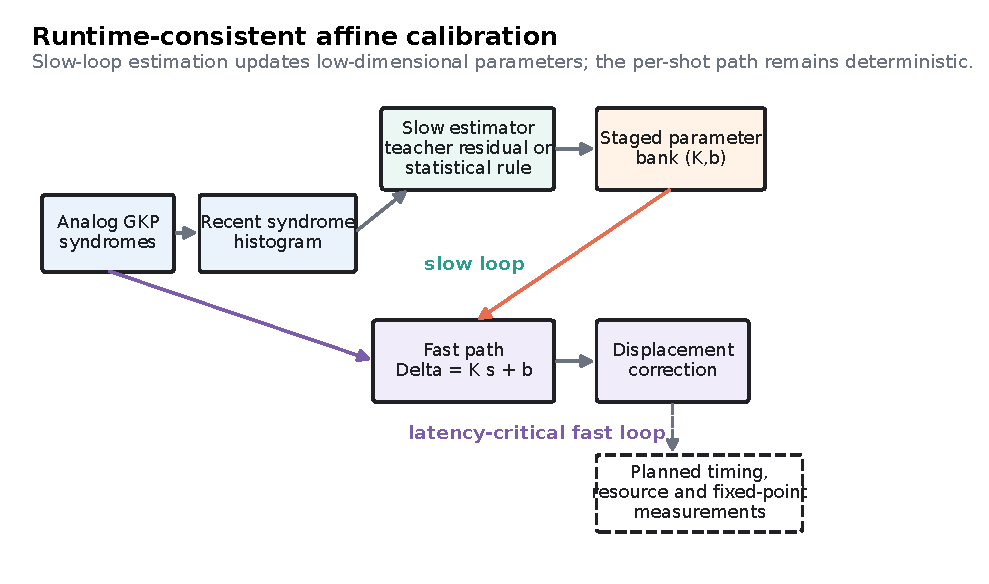
\includegraphics[width=0.95\linewidth]{fig01_dual_loop_architecture.pdf}
\caption{Overview of runtime-consistent affine calibration.  The slow
calibration loop updates low-dimensional \((K,b)\) parameters from recent
syndrome statistics, while the latency-critical fast path remains the
deterministic affine operation in Eq.~\eqref{eq:fastpath}.  The dashed
hardware-facing surface marks device timing, fixed-point and resource
measurements that are outside the present study.}
\label{fig:architecture}
\end{figure}

The main contributions are:
\begin{enumerate}
    \item A runtime-consistent formulation of drift-adaptive GKP decoding as
    affine calibration of \((K,b)\), with the per-shot correction constrained
    to Eq.~\eqref{eq:fastpath}.
    \item A residual branch, instantiated here with teacher anchoring in the
    main comparison, that predicts a bounded bias calibration term while
    leaving the fast path deterministic.
    \item A predeclared four-scenario \softwarehil{} evaluation showing that
    the hybrid residual branch ranks lowest by mean \finalLER{} in all tested
    scenarios under the two-repeat protocol, plus two scenario-level
    12-paired-repeat interval checks that strengthen the
    \texttt{static\_bias\_theta} and \texttt{linear\_ramp} rows without yet
    establishing an all-scenario interval result.
    \item A metric ladder separating protocol-defined
    \finalLER{}, residual-boundary channel language, analytical fast-path cost,
    fixed-point software parity and the hardware measurements needed before
    deployment-level claims.
    \item A comparison framework that positions the method against analog GKP
    decoding, adaptive-prior calibration, learned QEC modules and real-time
    FPGA decoders without treating incompatible metrics as a single
    leaderboard.
\end{enumerate}

\section{Related Work}

\paragraph{GKP analog information.}
Analog GKP syndrome values carry reliability information that can improve
decoding beyond hard thresholding.  Prior work has used analog information in
high-threshold GKP error correction, surface-GKP decoding and
bosonic-QLDPC-GKP settings \cite{fukui2018,noh2020,noh2022,raveendran2022,
berent2024,borah2025}.  The present work does not claim novelty in using
analog information.  Its distinction is the layer at which the information is
used: recent analog syndrome statistics update a physical-layer affine
displacement rule, rather than only an outer-code matching weight or message.
In other words, analog information is the established input class; the new
design question is where that information is committed in a hardware-facing
decoder stack.
The histogram window used here is also not a Bayesian multi-round approximate
GKP memory decoder and does not model noisy auxiliary-state correlations
\cite{wan2020,roy2025}.  It is an effective-noise calibration signal for a
committed physical affine surface.

\paragraph{Adaptive priors and calibration-aware decoding.}
Decoder performance depends on the match between assumed and actual noise.
Adaptive weight estimation, syndrome-statistics estimation and calibrated
decoders address this mismatch by updating priors or graph weights from
observed data \cite{spitz2018,wagner2021,dgr2023,chen2022,sivak2024}.  Our
formulation follows the same motivation, but constrains the updated object to
the GKP affine fast-path parameters and commits those parameters through a
stage-and-commit runtime contract.  The calibrated quantity is therefore not a
decoder score or graph edge alone, but the \((K,b)\) surface consumed by the
physical correction rule.

\paragraph{Learned low-latency QEC modules.}
Machine-learning-assisted decoders and pre-decoders can reduce latency or
improve accuracy when their role in a classical decoding stack is explicit
\cite{bausch2024,chamberland2026,stein2026,wang2022,peled2026,hanisch2026}.
Structured neural decoders, soft-information decoders and calibration-driven
control updates have also been studied in bosonic, surface-code and
hardware-data settings \cite{wang2022,peled2026,hanisch2026,sivak2026}.  The
residual module studied here is narrower than a full neural decoder: it
predicts a bounded calibration term for a low-dimensional affine surface and is
kept outside the per-shot critical path.  The novelty claim is therefore not
``neural GKP decoding'', but the restriction of adaptation to a committed
affine fast-path surface.
The closest learned-decoder contrasts are calibration-conditioned or real-time
neural modules, such as folded FiLM-style calibration and FPGA neural decoding
\cite{stein2026,yang2026}.  Those systems place learned computation closer to
the decoder or feedback path; here, learning is confined to slow-loop
calibration and the fast path remains an affine displacement rule.

\paragraph{Real-time and FPGA QEC decoders.}
Hardware QEC decoders for stabilizer-code settings include lookup-table,
union-find, matching-accelerator, clustering, greedy and FPGA-tailored
message-passing systems \cite{lilliput2022,helios2023,collision2025,
qldpcfpga2025,caune2024,yang2026,ziad2024,maurer2025}.  These
works define the standard for deployment claims: closed-loop latency,
resource use, timing closure and hardware integration.  This paper addresses a
different measurement layer: it treats the GKP affine fast-path contract as the
object to be isolated in controlled simulation and fixed-point software checks,
with hardware-facing metrics reserved for board-level implementation.
This distinction also fixes the comparison unit.  The prior FPGA systems
evaluate complete stabilizer-code decoding workloads and report device-level
timing, memory or integration evidence.  The present study evaluates a
physical-layer correction surface that would sit upstream of such a broader
decoder stack.  Its hardware relevance is therefore the compactness and
observability of the online rule: the affine update is small enough to be
fixed-point checked, logged and compared against a later source-vs-board test
target.
Hardware systems such as lookup-table, union-find, clustering and neural-FPGA
decoders report latency, resource, memory or closed-loop evidence as device
measurements \cite{lilliput2022,helios2023,collision2025,caune2024,yang2026};
this manuscript instead defines the affine target that such a measurement would
need to validate.

The closest prior-work cluster is therefore not a single decoder family, but
the intersection of three constraints: analog GKP reliability information,
adaptive noise or prior calibration, and real-time decoder implementation.
Existing GKP soft-information work establishes the value of continuous syndrome
data; adaptive-prior and calibration-conditioned decoders establish that
decoder parameters should track drift; and FPGA/QEC runtime work establishes
that deployment claims require bounded datapaths and measured latency.  The
present work is positioned at their intersection: it updates a physical-layer
affine correction surface while keeping the per-shot correction path
deterministic.

\begin{table}[t]
\centering
\small
\begin{tabular}{@{}>{\raggedright\arraybackslash}p{0.24\linewidth}>{\raggedright\arraybackslash}p{0.28\linewidth}>{\raggedright\arraybackslash}p{0.34\linewidth}@{}}
\toprule
Topic & Prior scope & Distinction of this work \\
\midrule
GKP analog decoding & Uses continuous syndrome values or reliability weights
for GKP or outer-code decoding. & Uses recent analog histograms to calibrate
the physical-layer affine displacement rule itself. \\
\addlinespace
Adaptive priors & Updates noise weights, graph weights or decoder priors from
syndrome statistics. & Maps the estimated state to committed \((K,b)\)
parameters consumed by a deterministic fast path. \\
\addlinespace
Learned QEC modules & Places neural modules before, inside or after a
classical decoder. & Keeps the neural branch in the slow calibration loop
rather than on the per-shot correction path. \\
\addlinespace
FPGA/real-time decoders & Reports deployed low-latency or hardware-integrated
decoders in stabilizer-code settings. & Provides a software-tested GKP
physical-layer calibration contract; hardware results require direct
board-level measurements. \\
\bottomrule
\end{tabular}
\caption{Topic-level positioning.  The contribution is the runtime-bounded
affine calibration contract for a drifting GKP physical correction layer, not
a dismissal of prior analog, learned or hardware-decoder work.}
\label{tab:related}
\end{table}

The comparison is metric-oriented rather than leaderboard-style.  Prior work
reports different code families, validation layers and endpoint metrics, so
Table~\ref{tab:closest-work-positioning} identifies the measurement standard
each line establishes and the narrower metric reported here; the expanded
literature crosswalk is provided in
Tables~\ref{tab:external-comparison} and~\ref{tab:external-runtime-comparison}
in the appendix.  We use three rules when reading these external numbers.
First, endpoint metrics are not exchanged across layers: surface-GKP
thresholds, logical-channel infidelities, real-processor LER and FPGA latency
are standards for comparison, not measurements produced by this study.  Second,
the adaptive object must be named: prior work often updates an outer-code
graph, a decoder prior, a neural decoder state or a message-passing likelihood,
whereas this manuscript updates the physical-layer affine surface \((K,b)\).
Third, the runtime surface must be separated from the estimator: the present
fast path remains a deterministic clipped affine rule even when the slow-loop
estimator is learned.

\begin{table}[t]
\centering
\scriptsize
\begin{tabular}{@{}>{\raggedright\arraybackslash}p{0.20\linewidth}>{\raggedright\arraybackslash}p{0.27\linewidth}>{\raggedright\arraybackslash}p{0.25\linewidth}>{\raggedright\arraybackslash}p{0.18\linewidth}@{}}
\toprule
Prior work class & Reported LER, fidelity, latency or resource metric & This work reports & Further validation needed \\
\midrule
Analog and surface-GKP decoding & Squeezing, failure and overhead anchors include about \(16.0\!\to\!9.8\) dB required squeezing, \(11.2/18.6\) dB and \(0.69/0.81\%\) threshold-type values, \(0.87\%\!\to\!0.36\%\) CNOT-failure reduction, and \(291\) modes plus \(97\) qubits versus \(1457\) qubits for a matched target \cite{fukui2018,noh2020,noh2022,berent2024,borah2025}. & A physical-layer affine calibration rule driven by recent GKP syndrome histograms and evaluated by a protocol-defined residual-boundary LER proxy. & End-to-end surface-GKP threshold, overhead or logical-channel failure rate. \\
\addlinespace
Calibration-aware and learned QEC decoders & Drift-aware graph and prior calibration report \(3.6\times\) average mismatch-LER reduction, worst-case reductions up to \(7360\times\), and prior-calibration gains of \(48\%\), \(16\%\) and \(3.3\%\); calibration-conditioned learned decoders report large-shot real-device studies and up to \(11.11\times\) LER reductions \cite{dgr2023,chen2022,sivak2024,bausch2024,stein2026}. & A learned slow-loop estimator for a low-dimensional affine surface; the per-shot GKP correction remains deterministic. & Real-processor learned-decoder LER, calibration-shot scaling or device-dataset generalization. \\
\addlinespace
Finite-energy logical-channel analyses & Logical-channel probabilities, channel infidelity and loss/amplification recovery curves include anchors such as GRN Pauli probabilities \(p_I=0.9900\), logical-channel infidelity curves and near-optimal loss/amplification comparisons \cite{jafarzadeh2025,hastrup2023,zheng2024}. & Residual-boundary event decompositions and a finite-squeezing toy-channel sanity check that connect the LER proxy to channel language. & Calibrated finite-energy logical-channel fidelity, channel infidelity or process tomography. \\
\addlinespace
Runtime pre-decoders and calibration-conditioned neural modules & Runtime anchors include \(270.83\!\to\!38.78\,\mu\mathrm{s}\) sub-step pre-decoding, \(85\)--\(95\,\mu\mathrm{s}\) folded FiLM latency, and real-time neural feedback examples with \(124\) ns neural decoding inside a 550 ns closed loop \cite{chamberland2026,stein2026,yang2026}. & An analytical fast path with four multiplications, four additions, no nonlinear operation and Q4.20 software parity in controlled samples. & Per-shot neural-decoder latency, closed-loop feedback latency or on-device FPGA timing. \\
\addlinespace
Real-time FPGA and hardware-tailored decoders & Hardware papers report \(28\)--\(42\) ns lookup latency, \(11.5\) ns/round FPGA decoding, \(810/240\) ns FPGA/ASIC collision decoding, sub-\(\mu\)s feedback paths, memory compression, area, power and source-to-device evidence \cite{lilliput2022,helios2023,qldpcfpga2025,caune2024,ziad2024,maurer2025,yang2026}. & A compact, fixed-point-checkable affine target with software runtime counters and explicit board-measurement requirements. & FPGA synthesis, LUT/FF/DSP/BRAM use, power, real-board latency and source-vs-board agreement. \\
\bottomrule
\end{tabular}
\caption{Closest-work metric comparison.  The table separates what adjacent
work reports, what this manuscript reports and which validation class is not
reported in this study.  The comparison is intentionally not a normalized leaderboard,
because the code families, physical endpoints and hardware-validation levels
differ.}
\label{tab:closest-work-positioning}
\end{table}

Taken together, the comparison defines a narrow but concrete advantage claim.
The manuscript does not compete with surface-GKP or QLDPC-GKP decoders on
end-to-end overhead, and it does not compete with real-time FPGA decoders on
measured device latency.  Instead, it tests whether drift adaptation can be
expressed as a small physical-layer affine update whose online arithmetic is
much simpler than posterior branch search while still improving the
protocol-defined LER proxy under controlled drift.  The closest adjacent
neural-FPGA demonstration is therefore a standard to validate against, not a
baseline that this study has already matched.  The design trade-off tested
here is architectural and decomposes into three parts:
the correction surface adapts under controlled drift, the latency-critical
operation remains a clipped affine matrix-vector rule, and the implementation
target is small enough to be checked against source-level vectors.  This gives
the manuscript a route to three later hardware-facing metrics: lower
analytical per-shot arithmetic count than the branch-aware posterior references
evaluated in the controlled cost model, a smaller source-level verification
target than a per-shot neural decoder and
a clear source-vs-board agreement target for an FPGA implementation.

This protocol also explains which comparisons are most probative for the
present claim.  Analog-GKP and calibration-aware QEC work establish that
continuous syndrome information and drifting calibration states matter.  They
do not by themselves establish a hardware-friendly physical correction
interface.  Learned-decoder and real-time-FPGA work establish the evidence bar
for LER and latency claims.  They do not remove the need for a small,
verifiable fast path when the goal is a GKP correction module that can later be
implemented with fixed-point arithmetic.  The contribution is therefore not a
new universal decoder, but a way to expose drift adaptation through a
low-dimensional surface whose online arithmetic, state and board-validation
interface are explicitly bounded.

For clarity, the manuscript uses a metric ladder rather than a single
all-purpose performance number.  The primary result is the protocol-defined
\finalLER{} ranking and paired descriptive delta.  The residual-boundary
surrogate is only a bridge from half-lattice crossing events to channel
language, not a finite-energy logical-channel fidelity.  The fast-path latency
argument is an analytical and software-emulation argument, not an FPGA timing
result.  Table~\ref{tab:metric-readiness} separates the metrics
reported in this study from the metrics that define the standard for later
validation.

\begin{table}[t]
\centering
\scriptsize
\begin{tabular}{@{}>{\raggedright\arraybackslash}p{0.20\linewidth}>{\raggedright\arraybackslash}p{0.24\linewidth}>{\raggedright\arraybackslash}p{0.23\linewidth}>{\raggedright\arraybackslash}p{0.21\linewidth}@{}}
\toprule
Metric axis & Manuscript metric & Supported statement & Missing for stronger claim \\
\midrule
Logical-error proxy & \finalLER{} means, paired descriptive deltas and a non-inferential paired-bootstrap envelope & Hybrid residual calibration has the lowest mean protocol-defined \finalLER{} in the tested drift scenarios. & More repeats, inferential confidence intervals, holdout drift and logical-channel reconstruction. \\
\addlinespace
Logical-channel fidelity & Residual-boundary Pauli-channel-style surrogate, method-level lattice sanity summary and finite-squeezing toy-channel sanity check & The surrogate links q/p half-lattice crossing rates to channel language, while the toy finite-squeezing check compares hard nearest-syndrome, fixed affine and oracle affine rules under a simplified noisy measurement channel; neither estimates finite-energy logical-channel fidelity or process infidelity. & Channel-specific calibrated finite-energy simulation or logical-channel tomography. \\
\addlinespace
Drift robustness & Four scenario rankings plus controlled local-Gaussian checks, holdout drift stress tests and a commit-lag sweep & Controlled stress diagnostics expose where stale commits help or fail under random-walk, burst/reset and faster-than-window settings; they do not establish trained-branch holdout robustness. & A formal predeclared expanded benchmark, repeat-expanded uncertainty estimates, trained-branch holdout validation and board-measured stale-parameter latency distributions. \\
\addlinespace
Fast-path cost and latency & Analytical per-shot operation count plus Q4.20 software parity & The affine correction has lower analytical arithmetic and state footprint than the wrapped-posterior references evaluated here, and fixed-point emulation introduces no residual-boundary crossing change in the controlled sample set. & FPGA synthesis, timing closure, resource and power measurements, source-vs-board agreement and board-level latency distribution. \\
\addlinespace
Hardware-facing validation & Measurement requirements only & The manuscript defines what must be measured before making hardware claims. & Board logs, bitstream or RTL hash, DMA evidence, commit reliability and source-vs-board vectors. \\
\bottomrule
\end{tabular}
\caption{Metric-readiness matrix for the manuscript.  The table separates
reported metrics from external standards and implementation-stage validation requirements;
it does not convert the \finalLER{} proxy into channel fidelity,
statistical significance or hardware latency.}
\label{tab:metric-readiness}
\end{table}

This ladder is the intended reading guide for all cross-paper comparisons in
the manuscript.  The three quantitative axes should be read as a triangulation,
not as interchangeable endpoints.  The \finalLER{} rows test whether adaptive
calibration changes the protocol-defined boundary-crossing rate under drift.
The residual-boundary surrogate then asks whether the same q/p events can be
reported in channel language without pretending to reconstruct a finite-energy
logical channel.  The operation-count and fixed-point rows ask whether the
resulting correction rule has the size and numerical stability expected of a
real-time datapath candidate.  A positive result on only one axis would be weak:
lower \finalLER{} without a channel-language bridge would be hard to compare
with GKP fidelity work, a surrogate fidelity without the \finalLER{} protocol
would be detached from the reported benchmark, and a low arithmetic count
without parity checks would not justify a hardware-facing claim.

\section{Problem Setting}

\subsection{Approximate GKP syndrome model}

The ideal square-lattice GKP code represents logical states as combs in phase
space.  In the position quadrature, \(|0_L\rangle\) and \(|1_L\rangle\)
occupy alternating lattice points separated by \(\sqrt{\pi}\), while
stabilizer periods are \(2\sqrt{\pi}\).  Approximate GKP states replace the
Dirac comb by finitely squeezed peaks with a finite-energy envelope, so both
state preparation and readout add continuous noise to the modular syndrome.
Equivalently, in a common oscillator normalization with
\([\hat q,\hat p]=i\), the ideal code is stabilized by \(2\sqrt{\pi}\)
translations in phase space, generated for example by
\(S_q=\exp(i2\sqrt{\pi}\hat q)\) and
\(S_p=\exp(-i2\sqrt{\pi}\hat p)\), while logical Pauli operations correspond
to half-period displacements such as
\(Z_L=\exp(i\sqrt{\pi}\hat q)\) and
\(X_L=\exp(-i\sqrt{\pi}\hat p)\).  Error correction therefore reduces
small displacement errors modulo the stabilizer lattice: residual shifts inside
one half cell are returned to the intended branch, whereas residual shifts
crossing a half-cell boundary are assigned to an adjacent logical branch.  The
simulation metric below is a software-level version of this modular decision,
not a reconstruction of the oscillator state.
For example, one may view an approximate position-basis codeword schematically
as
\begin{equation}
    |\widetilde{0}_L\rangle_q
    \propto
    \sum_{n\in\mathbb{Z}}
    \exp\!\left[-\frac{(2n)^2\pi}{2\Delta_{\mathrm{env}}^2}\right]
    \int \mathrm{d}q\,
    \exp\!\left[-\frac{(q-2n\sqrt{\pi})^2}{2\Delta_{\mathrm{pk}}^2}\right]
    |q\rangle ,
    \label{eq:approx-gkp-comb}
\end{equation}
with the odd lattice sites representing \(|\widetilde{1}_L\rangle_q\).  The
peak width \(\Delta_{\mathrm{pk}}\) represents finite squeezing and the broad
envelope \(\Delta_{\mathrm{env}}\) limits oscillator energy.  The same
description applies in the conjugate quadrature after the corresponding Fourier
rotation.  The exact envelope, normalization and circuit depend on the physical
preparation route, but the decoder-facing consequence is common: finite
squeezing turns a sharp lattice-cell decision into a tail probability near the
half-lattice boundary.  A small change in residual scale or bias can therefore
produce a disproportionately large change in boundary-crossing probability when
the residual distribution sits near that decision surface.

This is also why calibration is a physical-layer question rather than only a
machine-learning question.  The correction surface depends on the local
posterior induced by the approximate state, the readout chain and the drifted
effective displacement process.  Changes in peak width alter the probability
mass near the half-cell boundary; changes in mean bias shift the local branch
centre; and changes in covariance orientation alter which linear combination of
q/p syndromes is most predictive of the residual.  Thus a decoder that keeps a
fixed affine rule is fast but implicitly assumes that these effective moments
are stationary.  Runtime calibration instead treats the affine surface itself
as the slowly changing object to be estimated from recent analog syndrome
statistics.

This tail sensitivity is the link between approximate-state physics and the
software metric used below.  In the usual Gaussian peak approximation, modular
squeezing can be summarized by a width parameter such as
\(S=-10\log_{10}\Delta_{\mathrm{pk}}^2\), while the finite-energy envelope
controls how much probability leaks into distant lattice peaks.  After a
syndrome measurement and correction, a residual \(r_j^+\) that remains well
inside the local cell is still compatible with the intended logical branch; a
residual that crosses \(\pm\lambda/2\) changes the nearest branch assignment.
For a zero-mean Gaussian residual with variance \(\sigma_r^2\), the corresponding
one-quadrature crossing probability is approximately
\(2Q(\lambda/(2\sigma_r))\), where \(Q\) is the Gaussian upper-tail function,
so modest changes in residual scale become
exponentially visible near the boundary.  This is why a drift-adaptive affine
surface can matter even when its correction rule is simple: it shifts the
post-correction residual distribution away from the cell edge rather than
attempting to reconstruct the full finite-energy wavefunction.

This finite-energy picture also fixes the level of abstraction used in the
paper.  The ideal code treats displacements separated by a stabilizer period as
equivalent, whereas an approximate code supplies only a noisy, periodic
measurement of the displacement.  The decoder therefore does not observe the
absolute shift \(e_t\).  It observes a modular residual together with
preparation, ancilla and readout noise, then chooses a correction that is safe
only within the selected lattice cell.  In this manuscript, a q or p event is
counted when the post-correction residual crosses the half-period boundary of
that normalized cell.  This is the operational origin of the reported
\finalLER{} proxy and of the later Pauli-style surrogate tables.

Two consequences of the approximate-code model are important for interpreting
the affine decoder.  First, finite squeezing makes branch assignment
probabilistic even when the correction rule is deterministic: a residual that is
small in Euclidean norm can still have non-negligible tail mass across the
nearest half-cell boundary.  Second, the wrapped syndrome aliases different
lattice branches, so a fast decoder that commits to one local branch must be
judged by the residual it leaves after correction, not by whether it has
reconstructed the global displacement.  The affine surface in this paper is
therefore a branch-local correction rule for an effective approximate-GKP
residual process.  It is not a statement that finite-energy GKP decoding is
globally affine, and it is not a replacement for a channel-level simulation of
prepared approximate codewords.

The syndrome readout is therefore modular rather than absolute.  If a
pre-correction displacement \(e_j\) occurs in quadrature \(j\in\{q,p\}\), the
readout exposes \(e_j\) only modulo the lattice period and with additive
preparation and measurement uncertainty.  The correction is successful within
the modeled cell when the post-correction residual
\(r_{j,t}^{+}\) remains inside the interval
\([-\lambda/2,\lambda/2)\).  The manuscript's per-round event indicator can be
written as
\begin{equation}
    \ell_t
    =
    \mathbb{1}\{|r_{q,t}^{+}|\ge \lambda/2\ \mathrm{or}\
    |r_{p,t}^{+}|\ge \lambda/2\},
    \label{eq:boundary-indicator}
\end{equation}
and \finalLER{} is the empirical mean of this indicator under the stated
software protocol.  This definition is intentionally narrower than a
code-distance logical failure probability: it measures whether the physical
fast-path correction leaves the residual in the wrong normalized cell, not
whether an outer code or a full finite-energy logical channel has failed.

To avoid mixing oscillator and software coordinates, the remainder of the paper
uses one normalized residual convention.  The conventional square-lattice GKP
description above explains the physical code.  The runtime equations below use
the software residual coordinate in which the wrap period is
\(\lambda=\sqrt{2\pi}\).  All q/p crossings, clipping thresholds and source
tables are expressed in that normalized coordinate.

\begin{table}[htbp]
\centering
\small
\begin{tabular}{@{}>{\raggedright\arraybackslash}p{0.24\linewidth}>{\raggedright\arraybackslash}p{0.33\linewidth}>{\raggedright\arraybackslash}p{0.27\linewidth}@{}}
\toprule
Quantity & Meaning in the manuscript & Not claimed here \\
\midrule
Conventional GKP spacing & Used to introduce the ideal square-lattice code and
finite-energy comb picture. & A calibrated device-specific quadrature scale. \\
\addlinespace
\(\lambda=\sqrt{2\pi}\) & Software residual wrap period used by the emulator,
tables and supporting-data checks. & A new physical code definition. \\
\addlinespace
\(\lambda/2\) boundary & Normalized q/p half-cell boundary for the event
indicator in Eq.~\eqref{eq:boundary-indicator}. & Outer-code logical failure
probability. \\
\addlinespace
\finalLER{} & Empirical mean of residual half-cell crossings under the stated
runtime-calibration protocol. & Finite-energy logical-channel fidelity,
process fidelity or tomography. \\
\bottomrule
\end{tabular}
\caption{Coordinate and metric convention.  The table separates the physical
GKP motivation from the normalized software residual coordinate used in the
reported runtime-calibration benchmark.}
\label{tab:gkp-coordinate-convention}
\end{table}

Let the accumulated two-quadrature displacement before correction be
\(e_t=(e_{q,t},e_{p,t})^\top\).  The implementation uses the lattice period
\(\lambda=\sqrt{2\pi}\) for syndrome wrapping and half-lattice residual
boundaries.  A compact measurement model is
\begin{equation}
    \tilde{s}_t = \mathrm{wrap}_{[-\lambda/2,\lambda/2)}(e_t)
    + \eta_t^{\mathrm{meas}}+\eta_t^{\mathrm{GKP}} .
\end{equation}
The two noise terms summarize effective readout and finite-squeezing
contributions in the software model.  They are not fitted to a calibrated
finite-energy GKP device channel in this study.
The constant \(\lambda\) should be read as the coordinate convention used by
the software residual model, not as a new physical code definition.  Standard
GKP presentations often describe logical separation and stabilizer periods in
the oscillator quadrature normalization natural to the preparation circuit.
Here all measured syndromes, accumulated residuals and logical-boundary tests
are expressed in a normalized two-quadrature residual coordinate with period
\(\sqrt{2\pi}\).  This convention makes the runtime rule and the supporting data
unambiguous: every wrap, clipping threshold and boundary-crossing event in the
manuscript is evaluated against the same \(\lambda\), while squeezing in dB,
photon number and channel-specific finite-energy parameters remain outside the
present calibrated model.
Equivalently, the manuscript works after a fixed coordinate rescaling from the
usual oscillator-quadrature convention into the software residual coordinate;
all reported q/p crossings are crossings of this normalized cell, not separate
claims about a device-specific physical quadrature calibration.
The wrap operation is the essential ambiguity: the same reported syndrome can
correspond to different lattice branches.  If the posterior mass is
concentrated near one branch, a local affine estimator is a reasonable
low-latency approximation.  For jointly Gaussian local variables \(e\) and
\(s\), the linear-MMSE estimate is
\begin{equation}
    \hat e = \mu_e + \Sigma_{es}\Sigma_{ss}^{-1}(s-\mu_s)
    = Ks+b,\qquad
    K=\Sigma_{es}\Sigma_{ss}^{-1},\quad
    b=\mu_e-K\mu_s .
\end{equation}
This derivation motivates the affine fast path while also defining its
limits.  More explicitly, fix a lattice branch
\(m_t\in\mathbb{Z}^2\) and define the unwrapped local residual
\(r_t=e_t-\lambda m_t\).  Conditional on the effective noise state
\(\theta_t^{\mathrm{noise}}\) and on this branch assignment, suppose the local
pair \((r_t,s_t)\) is approximated by a joint Gaussian with moments
\((\mu_r,\mu_s,\Sigma_{rs},\Sigma_{ss})\).  The minimum-mean-square affine
correction is then
\begin{equation}
    \hat r_t
    =\mathbb{E}[r_t\mid s_t,\theta_t^{\mathrm{noise}},m_t]
    \approx \mu_r+\Sigma_{rs}\Sigma_{ss}^{-1}(s_t-\mu_s)
    = K(\theta_t)s_t+b(\theta_t).
\end{equation}
The affine rule used by the fast path is therefore not introduced as a
universal wrapped decoder.  It is the single-branch local conditional-mean
surface that remains after the slow loop has compressed recent syndrome
statistics into a small committed parameter bank.  The scientific question in
this paper is whether such a surface can remain useful under controlled drift
while preserving a deterministic low-latency datapath.
With the sign convention used in the emulator, the affine output is the
correction displacement applied to the pre-correction shift.  The post-correction
local residual is
\begin{equation}
    r_t^{+}=e_t-\Delta_t-\lambda m_t,\qquad
    \Delta_t=K_t s_t+b_t ,
    \label{eq:post-correction-residual}
\end{equation}
where \(m_t\) is the selected lattice branch.  Boundary events in the metric
section are defined on \(r_t^{+}\), so the affine surface is judged by the
residual it leaves after correction rather than by parameter error alone.

\begin{proposition}[Local affine fast path]
Fix an effective noise state \(\theta\) and a lattice branch \(m\).  Let
\((r,s)\) denote the corresponding unwrapped local residual and wrapped
syndrome, with finite second moments and nonsingular \(\Sigma_{ss}\).  Among
all affine corrections \(a(s)=As+c\), the unique minimum-mean-square
correction is
\[
    A^\star=\Sigma_{rs}\Sigma_{ss}^{-1},\qquad
    c^\star=\mu_r-A^\star\mu_s .
\]
If \((r,s)\) is jointly Gaussian within this conditioned branch, this affine
rule is also the conditional mean \(\mathbb{E}[r\mid s,\theta,m]\).
\end{proposition}

\begin{proof}
For an affine correction \(a(s)=As+c\), the mean-square risk is
\(\mathbb{E}\|r-As-c\|_2^2\).  Differentiating with respect to \(c\) gives
\(c=\mu_r-A\mu_s\).  Substituting the centred variables
\(\bar r=r-\mu_r\) and \(\bar s=s-\mu_s\), the remaining risk is
\(\mathbb{E}\|\bar r-A\bar s\|_2^2\).  The normal equations are
\(A\Sigma_{ss}=\Sigma_{rs}\), which yields
\(A^\star=\Sigma_{rs}\Sigma_{ss}^{-1}\) when \(\Sigma_{ss}\) is nonsingular.
For a jointly Gaussian pair, the conditional mean is linear with the same
coefficient and intercept.
\end{proof}

The proposition is intentionally local.  It justifies the committed
\((K,b)\) surface as the optimal affine correction after a branch and an
effective noise state have been compressed by the slow loop.  It does not
claim global optimality for wrapped, multi-branch posteriors, nor does it
replace a finite-energy logical-channel simulation.  Its role is to make the
runtime contract mathematically explicit: a slow estimator may update the
moments or their learned proxy, while the fast path only evaluates the affine
map fixed by the proposition.

This problem setting is deliberately weaker than a full logical-channel
simulation.  A complete approximate-GKP analysis would track finite-energy
envelopes, auxiliary-state noise, channel-specific loss or amplification, and
the induced logical Pauli channel.  The present model instead treats these
effects through an effective wrapped displacement process and asks whether a
runtime-constrained correction surface can adapt to controlled nonstationarity.
That restriction makes the FPGA-facing question concrete: the fast path
receives a wrapped syndrome and a committed affine parameter bank, not a full
posterior over lattice branches.

The separation is important for comparing with fidelity-oriented GKP work.
Channel-level studies ask how a physical loss, amplification or finite-energy
model propagates to logical probabilities or process infidelity.  This
manuscript asks a narrower systems question: if the physical correction layer is
restricted to a committed affine rule, can recent syndrome statistics keep that
rule aligned with a drifting effective residual distribution?  The answer is
reported with a half-lattice boundary proxy and diagnostic channel-language
surrogates.  It should not be interpreted as logical-channel fidelity because
the supporting data do not reconstruct the finite-energy output state or a
complete logical process map.

The validity regime can be stated in operational terms.  Let \(B_t\) be the
event that the wrapped syndrome is assigned to the wrong lattice branch after
conditioning on the recent histogram, and let \(c\) be the slow-loop update
window.  The affine path is expected to be useful when
\(\Pr(B_t\mid H_{t-c+1:t})\) is small, the local covariance of the conditioned
residual is well described by a single mode, and the drift timescale is long
enough that \((K_t,b_t)\) remains informative between commits.  It is expected
to fail when posterior mass splits across adjacent lattice branches, when
finite-energy tails place substantial probability near half-lattice
boundaries, or when drift changes faster than the histogram window and commit
cadence can track.  These three failure modes motivate the paper's bounded
evidence ladder: residual-MSE checks for local affine fit, boundary-crossing
\finalLER{} for branch-cell errors, holdout drift stress tests for slow-loop
lag and a hardware-facing datapath contract for device validation.  The
controlled oracle and wrapped-Gaussian analyses in the Results section test
this local validity regime rather than replacing a full wrapped decoder
benchmark.

\subsection{Effective drift state}

The slow loop estimates a compact effective noise state rather than a full
circuit-level model:
\begin{equation}
    \theta_t^{\mathrm{noise}}
    =(\sigma_t,\mu_{q,t},\mu_{p,t},\vartheta_t).
\end{equation}
Here \(\sigma_t\) summarizes displacement scale, \(\mu_{q,t}\) and
\(\mu_{p,t}\) represent mean bias, and \(\vartheta_t\) captures covariance
orientation.  The benchmark uses four hand-designed drift families:
static bias with rotation, linear ramp, step change in variance/orientation
and periodic drift.  These scenarios test distinct adaptation demands but do
not exhaust possible nonstationary GKP noise.

\subsection{Evaluation target}

The primary metric is \finalLER{}, the reported table field for a q/p
boundary-crossing count per fast-loop round.  Lower values are better.  Because
the main comparison table does not include confidence intervals or a formal
predeclared holdout set, the main result is interpreted as a predeclared-protocol
ranking, not as a broad distributional generalization claim.  Controlled holdout
stress tests are reported separately in the Results section, and
repeat-expanded inferential confidence intervals or predeclared bootstrap
intervals for the main rows remain required before
stronger statistical language is appropriate.

\begin{center}
\fbox{\begin{minipage}{0.92\linewidth}
\textbf{Metric definition.}
For one \softwarehil{} run, \texttt{final\_ler} is the final value of the
cumulative q/p residual-boundary crossing proxy reported by the fast-loop
emulator,
\[
    \texttt{final\_ler}=\frac{N_X+N_Z}{T},
\]
where \(N_X\) and \(N_Z\) are the numbers of q- and p-quadrature residual
boundary crossings counted by \texttt{LogicalErrorTracker}, and \(T\) is the
number of fast-loop rounds in the run.  The table field \finalLER{} is the
mean of this value across the available repeats for each scenario and mode;
the associated \texttt{final\_ler\_sd} field is a descriptive standard
deviation.  Because q and p crossings are counted separately, simultaneous
crossings contribute two events; the field is therefore an event-count proxy,
not a probability bounded by one.  This definition is a \softwarehil{} protocol
metric.  It is not a hardware logical-error measurement, a logical-channel
estimate, a confidence interval or a significance test.
\end{minipage}}
\end{center}

The proxy follows the standard GKP intuition that a residual displacement past
the half-lattice boundary corresponds to a logical branch error in the
associated quadrature.  Counting q- and p-boundary crossings therefore gives a
software-level indicator of how often the fast path leaves the residual on the
wrong side of the correctable cell.  It does not capture the full logical
channel, correlations across repeated correction rounds, leakage, auxiliary
state noise or outer-code behavior.  Those omissions are why the metric is
reported as \finalLER{} rather than as logical-channel fidelity or hardware
logical-error rate.

The relation between the reported proxy and the channel-style surrogate can be
made explicit.  For round \(t\), define
\[
    X_t=\mathbb{1}\{|r_{q,t}|>\lambda/2\},\qquad
    Z_t=\mathbb{1}\{|r_{p,t}|>\lambda/2\},
\]
where \(r_{q,t}\) and \(r_{p,t}\) are the components of
\(r_t^{+}\) in Eq.~\eqref{eq:post-correction-residual}.  The reported
run-level proxy is
\[
    \texttt{final\_ler}=\frac{1}{T}\sum_{t=1}^T (X_t+Z_t).
\]
The union event used in the surrogate channel table is
\[
    U_t=\mathbb{1}\{X_t\lor Z_t\}=X_t+Z_t-X_tZ_t .
\]
Thus \(\mathbb{E}[U_t]\) and \(\mathbb{E}[X_t+Z_t]\) are linked but not
identical: a simultaneous q/p crossing contributes once to \(U_t\) and twice to
\finalLER{}.  In expectation, \(p_{\mathrm{any}}\le
\mathbb{E}[X_t+Z_t]\le 2p_{\mathrm{any}}\).  This is why the manuscript reports
\finalLER{} as the primary software metric and uses the surrogate channel
language only as an interpretive bridge from boundary events to Pauli-like
categories.  A genuine finite-energy logical-channel fidelity would require
propagating the corrected approximate-GKP state or an equivalent logical
process map, not only counting residual boundary events
\cite{jafarzadeh2025,hastrup2023,zheng2024}.

\subsection{Boundary sensitivity and surrogate channel language}

The half-lattice boundary also gives a compact theoretical bridge between
residual-scale metrics and channel-style language.  If a residual quadrature is
approximated locally as \(r\sim\mathcal{N}(0,\sigma_r^2)\), the probability of a
single-quadrature boundary crossing is
\begin{equation}
    p_{\mathrm{cross}}(\sigma_r)=
    \mathrm{erfc}\!\left(\frac{\lambda/2}{\sqrt{2}\sigma_r}\right).
\end{equation}
Assuming independent q and p residuals with the same local scale gives
\begin{equation}
    p_{\mathrm{any}} = 1-(1-p_{\mathrm{cross}})^2 .
\end{equation}
This calculation is not a finite-energy logical-channel simulation.  It is a
diagnostic bridge: it explains why residual variance near the decision
boundary can change a boundary-crossing metric sharply, and why \finalLER{} and
residual MSE are related but not interchangeable.

\begin{table}[htbp]
\centering
\small
\begin{tabular}{@{}rrrrr@{}}
\toprule
\(\sigma_r\) & Eq. squeezing (dB) & \(p_{\mathrm{cross}}\) & \(p_{\mathrm{any}}\) & Surrogate infidelity \\
\midrule
0.15 & 16.48 & 0.000000 & 0.000000 & 0.000000 \\
0.20 & 13.98 & 0.000000 & 0.000000 & 0.000000 \\
0.25 & 12.04 & 0.000001 & 0.000001 & 0.000001 \\
0.30 & 10.46 & 0.000029 & 0.000059 & 0.000039 \\
0.35 & 9.12 & 0.000342 & 0.000685 & 0.000456 \\
0.40 & 7.96 & 0.001729 & 0.003454 & 0.002303 \\
\bottomrule
\end{tabular}
\caption{Analytical residual-boundary sensitivity for a zero-mean Gaussian
residual model.  The equivalent squeezing column is
\(-10\log_{10}\sigma_r^2\).  The surrogate infidelity is
\(1-(1+2(1-p_{\mathrm{any}}))/3\), used only to connect boundary events to
channel-style terminology; it is not a finite-energy GKP logical-channel
fidelity or process-infidelity estimate.}
\label{tab:gkp-boundary-sensitivity}
\end{table}

\subsection{Metric interpretation}

The notation above is tied to a concrete implementation, but only at
the level needed for a scoped protocol claim.  The implementation underlying the
reported tables uses the same GKP lattice constant \(\lambda=\sqrt{2\pi}\) for
syndrome wrapping, half-lattice logical boundaries and fast-loop histogram
limits.  The measurement model
includes finite-energy and readout terms through a compact configuration, and
the fast-loop emulator records residual accumulation with the same half-lattice
logical-error rule.  These anchors support the statement that \finalLER{} is a
protocol-defined logical-error proxy for the present \softwarehil{} setting.
They do not turn the benchmark into a full finite-energy GKP physical
model, a wrapped-posterior decoder comparison, a holdout drift distribution or
a hardware measurement.  The present supporting-data checks are consistency
checks between manuscript tables, implementation outputs and generated figures; they are
not physical validation.

\begin{table}[htbp]
\centering
\small
\begin{tabular}{@{}>{\raggedright\arraybackslash}p{0.20\linewidth}>{\raggedright\arraybackslash}p{0.30\linewidth}>{\raggedright\arraybackslash}p{0.22\linewidth}>{\raggedright\arraybackslash}p{0.16\linewidth}@{}}
\toprule
Object & Current support & Manuscript use & Missing before stronger claim \\
\midrule
Syndrome wrapping &
Shared \(\sqrt{2\pi}\) lattice constant and wrap interval
\([-\lambda/2,\lambda/2)\). &
Approximate GKP syndrome model. &
Independent symbol-to-code validation. \\
\addlinespace
Finite-energy and measurement noise &
Configurable \(\Delta\), measurement efficiency, shot noise and ancilla-error
terms in the software measurement model. &
Approximate measurement effects only. &
Full physical-noise calibration. \\
\addlinespace
Effective drift &
Synthetic \((\sigma,\mu_q,\mu_p,\vartheta)\) trajectories drive the
\softwarehil{} protocol. &
Controlled drift probes. &
Unseen or device-derived drift families. \\
\addlinespace
\finalLER{} &
Residual accumulation is scored against half-lattice logical boundaries in the
fast-loop emulator. &
Predeclared-protocol logical-error proxy. &
Logical-channel validation and stronger baselines. \\
\addlinespace
Hardware path &
Board-facing rows specify required device-measurement classes. &
Board-validation target. &
Measured device logs and resource/timing data. \\
\bottomrule
\end{tabular}
\caption{Physics-model and metric scope.  The implementation
anchors the notation used in the paper, but the evidence supports only a
\softwarehil{} protocol claim.}
\label{tab:physics-metric-boundary}
\end{table}

\section{Method}

\subsection{Overview}

The method decomposes drift-adaptive correction into three modules
(Fig.~\ref{fig:architecture}).  The fast path applies the active affine
correction.  The teacher or calibration module estimates a low-dimensional
noise state from recent histograms.  The runtime controller stages, clips,
smooths and commits candidate parameters into the bank consumed by the fast
path.

Each module has a distinct scientific and engineering role.  The fast path is
the object that must eventually meet a hard timing budget, so it is deliberately
limited to clipping, fixed-point arithmetic, a \(2\times2\) matrix-vector
operation and status logging.  The slow estimator is the object that absorbs
nonstationarity, so it is allowed to use windowed histograms, teacher features
or statistical summaries unavailable to a single-shot combinational datapath.
The runtime controller is the safety interface between them: it prevents an
unstable estimate from becoming an active correction until the candidate
surface has passed clipping, quantization and commit checks.  This separation
lets the paper compare estimator families without changing the timing-critical
operation being validated.

\subsection{Design rationale and testable predictions}

The design is useful only if it makes stronger claims easier to test.  The
central hypothesis is not that an affine rule is a complete GKP decoder, but
that the adaptive state of a drift-aware physical correction layer can be
compressed into a small surface whose online arithmetic is deterministic.  This
compression creates four testable predictions.  First, if drift mainly changes
local bias, scale or orientation, recent syndrome statistics should improve the
committed \((K,b)\) surface and lower residual-boundary events relative to a
static or slowly mismatched affine reference.  Second, if the estimator is kept
outside the per-shot path, the online cost should scale with the affine
datapath rather than with posterior branch count or neural-network depth.
Third, if the same committed state is logged in software and hardware, a board
implementation should be checkable by source-vs-board vectors
rather than by only aggregate logical-error rates.  Fourth, if the local
single-branch assumption fails, the method should fail in identifiable ways:
posterior mass should split across lattice branches, half-lattice crossings
should increase, or stale parameters should dominate the commit-lag sweep.

These predictions determine how the experiments are organized.  The main
\softwarehil{} benchmark tests the first prediction under four controlled
drift families.  The analytical cost model and Q4.20 parity check test the
second prediction at the software and arithmetic-contract level.  The runtime
counters and validation-contract figure make the third prediction observable,
although board measurements are still absent.  The oracle-affine,
wrapped-Gaussian, holdout-stress and commit-lag diagnostics address the fourth
prediction by showing when local affine tracking is plausible and where it
should be distrusted.  This rationale is the reason the manuscript reports
multiple bounded metrics instead of converting them into a single headline
score.

\begin{table}[t]
\centering
\small
\begin{tabular}{@{}>{\raggedright\arraybackslash}p{0.23\linewidth}>{\raggedright\arraybackslash}p{0.31\linewidth}>{\raggedright\arraybackslash}p{0.30\linewidth}@{}}
\toprule
Design prediction & Supporting observation in this study & Observation that would weaken the claim \\
\midrule
Slow calibration can track drift without changing the fast-path rule. &
The hybrid residual branch has the lowest mean protocol-defined \finalLER{} in
the four controlled drift scenarios, and two scenario-level 12-pair checks
support positive UKF-minus-hybrid intervals. &
The same advantage disappearing under repeat expansion, trained-branch holdout
drift, or matched known-noise baselines. \\
\addlinespace
The latency-critical rule remains small enough to be a hardware target. &
The online rule is a clipped \(2\times2\) affine map with four multiplications,
four additions and six stored state scalars, plus Q4.20 software parity in the
controlled sample set. &
FPGA synthesis showing poor timing closure, excessive routing/resource cost, or
source-vs-board mismatch under the same committed \((K,b)\) traces. \\
\addlinespace
The contract is estimator-agnostic rather than CNN-specific. &
Feature ablations constrain the neural mechanism story, and a supplementary
statistical-calibration analysis can populate the same affine interface. &
A matched protocol showing that only one neural feature set works, or that
non-neural calibration fails once candidate generation and selection are fixed. \\
\addlinespace
The affine model has identifiable validity limits. &
Oracle-affine, wrapped-Gaussian, holdout-stress and commit-lag diagnostics expose
branch-local headroom, posterior-branch brittleness and stale-parameter regimes. &
A full nearest-lattice or sequence-level wrapped decoder dominating the affine
path across the same drift settings without increasing fast-path cost. \\
\bottomrule
\end{tabular}
\caption{Falsification-oriented design logic for the affine runtime contract.
Each claimed advantage is paired with both the present supporting observation
and a concrete observation that would weaken or overturn the claim.  The table
is a roadmap for interpreting the Results rather than an additional experiment.}
\label{tab:falsification-design}
\end{table}

\subsection{Algorithmic protocol}

The protocol-level object is a sequence of committed affine surfaces rather
than a single neural prediction.  At each slow-loop update, the implementation
uses the recent syndrome window \(H_{t-c+1:t}\), its time differences and any
available teacher or statistical state to propose a candidate
\((K_t^{\mathrm{cand}},b_t^{\mathrm{cand}})\).  The candidate is clipped,
optionally smoothed, checked against fixed-point and saturation limits, and
staged in an inactive parameter bank.  A commit event makes the candidate the
active surface only at a safe epoch boundary.  Between two such commits, every
shot uses the same active surface through Eq.~\eqref{eq:fastpath}.

This organization makes the estimator interchangeable but keeps the fast-loop
contract fixed.  A teacher-anchored residual branch, a statistical calibration
rule or another estimator may differ in how it proposes
\((K_t^{\mathrm{cand}},b_t^{\mathrm{cand}})\), but the logged runtime state is
the same: active \(K,b\), staged \(K,b\), clipping and saturation status,
commit acknowledgement, stale-parameter counters and the resulting residual
boundary events.  These fields are the minimum information needed to reproduce
the software protocol and to compare a board implementation against the
same source trajectory.  The present manuscript evaluates this protocol in
software; it does not report board commit latency or source-vs-board agreement.

\begin{table}[htbp]
\centering
\small
\begin{tabular}{@{}>{\raggedright\arraybackslash}p{0.12\linewidth}>{\raggedright\arraybackslash}p{0.30\linewidth}>{\raggedright\arraybackslash}p{0.42\linewidth}@{}}
\toprule
Step & Operation & Reproducible state recorded by the protocol \\
\midrule
1 & Accumulate recent syndrome statistics. &
Windowed histogram \(H_{t-c+1:t}\), histogram differences, active scenario
index and fast-loop shot count. \\
\addlinespace
2 & Propose a candidate affine surface. &
Candidate \(K_t^{\mathrm{cand}}\), \(b_t^{\mathrm{cand}}\), estimator family
and any teacher or statistical state used to compute the proposal. \\
\addlinespace
3 & Apply runtime guards before exposure to the fast path. &
Clipped and optionally smoothed \(K,b\), saturation flags, overflow flags and
the inactive bank selected for staging. \\
\addlinespace
4 & Commit only at a safe update boundary. &
Commit acknowledgement, active-bank selector, stale-parameter counter and
rollback status. \\
\addlinespace
5 & Correct every shot with the committed affine rule. &
Clipped syndrome, quantized correction, residual displacement and q/p
half-lattice boundary indicators. \\
\bottomrule
\end{tabular}
\caption{Reproducible algorithmic contract for affine runtime calibration.
Different slow-loop estimators may populate the candidate surface, but all
paths must expose the same committed \(K,b\) state and the same fast-loop log
fields.  These fields are sufficient for the software comparisons reported
here and define the source-vs-board trace needed for hardware
validation.}
\label{tab:algorithmic-contract}
\end{table}

\subsection{Affine fast path}

Given the measured syndrome \(s_t\), the fast path computes
\begin{align}
    s_t^{\mathrm{clip}} &= \mathrm{clip}(s_t,-s_{\max},s_{\max}),\\
    \Delta_t^{\mathrm{raw}} &= K_t s_t^{\mathrm{clip}} + b_t,\\
    \Delta_t &= Q\!\left(
    \mathrm{clip}(\Delta_t^{\mathrm{raw}},-\Delta_{\max},\Delta_{\max})
    \right),
\end{align}
where \(Q(\cdot)\) denotes fixed-point quantization.  A hardware
implementation can represent \(K_t\), \(b_t\), clipped syndromes and residual
corrections in a selected \(Q_{m,n}\) format, expose saturation flags, and
route the active parameter bank through a small matrix-vector datapath.  The
fast-path latency model is correspondingly simple:
\begin{equation}
    L_{\mathrm{fast}} =
    L_{\mathrm{wrap}}+L_{\mathrm{matvec}}+L_{\mathrm{clip}}+L_{\mathrm{bank}} .
\end{equation}
This module is needed because the per-shot QEC path must remain small enough
for deterministic execution and independent validation.  Its advantage is not
that affine decoding is globally optimal, but that all more complex estimation
can be moved outside the fast timing boundary.

The latency budget has two different meanings in this contract.  The
correction latency is the shot-local delay for wrapping, clipping, matrix-vector
evaluation and output registration.  The update or commit latency is the delay
with which a newly estimated \((K,b)\) bank becomes active.  Only the first
latency lies directly on the per-shot correction path; the second appears as a
stale-parameter effect and is therefore probed separately by the commit-lag and
runtime-counter diagnostics.  Separating these two clocks is essential for a
hardware implementation: a slower CNN, teacher or statistical estimator can be
acceptable only if its output is staged and committed without perturbing the
deterministic correction cycle.

The latency expression is meant as a design decomposition rather than a board
measurement.  A fully parallel implementation can assign four fixed-point
multipliers to the \(2\times2\) product and reduce the matrix-vector stage to a
short adder tree plus output registers.  A resource-minimal implementation can
reuse fewer multipliers across several cycles, increasing
\(L_{\mathrm{matvec}}\) while reducing DSP use.  Both realizations execute the
same committed map and can be checked by the same tuple stream.  This is the
main hardware-facing benefit of the formulation: latency and area can be traded
by changing the arithmetic schedule without changing the estimator, the
scientific metric or the source trace.

\begin{table}[htbp]
\centering
\small
\begin{tabular}{@{}>{\raggedright\arraybackslash}p{0.24\linewidth}>{\raggedright\arraybackslash}p{0.30\linewidth}>{\raggedright\arraybackslash}p{0.30\linewidth}@{}}
\toprule
Datapath assumption & Parallel schedule & Serialized schedule \\
\midrule
Numeric format & Q4.20 fixed-point words, matching the software parity check. &
Same Q4.20 source-vector format. \\
\addlinespace
Multiplier allocation & Four fixed-point multipliers for the \(2\times2\)
product. & One or two multipliers reused across the four products. \\
\addlinespace
Cycle model & Product stage followed by add, bias, clip and register stages;
clock period not claimed. & More arithmetic cycles, with the same input and
output tuple stream; clock period not claimed. \\
\addlinespace
Active state & Six affine words (\(K,b\)) plus clip thresholds, bank selector
and status flags. & Same state; lower multiplier footprint changes schedule,
not protocol state. \\
\addlinespace
Validation target & Match source corrections and flags within declared
fixed-point tolerance. & Same source-vs-board target. \\
\bottomrule
\end{tabular}
\caption{Pre-synthesis datapath assumptions for the affine fast path.  The
table states the implementation model that motivates the operation-count and
fixed-point checks.  It is not synthesis, timing closure, resource measurement
or a board result.}
\label{tab:presynthesis-datapath-assumptions}
\end{table}

\subsection{FPGA-facing datapath contract}

The hardware-facing object in this study is a datapath contract, not a
measured device implementation.  The contract has five parts: a wrapped
two-quadrature syndrome input; an active bank containing \(K_t\), \(b_t\) and
clip thresholds; a fixed-point affine matrix-vector operation; a corrected
displacement output; and status flags for clipping, overflow, stale parameters
and bank commits.  This decomposition is useful because every fast-path output
can be checked against a software reference with explicit input vectors and
parameter-bank state.  It also makes the negative comparison precise: a
per-shot wrapped-posterior decoder must evaluate multiple branch hypotheses
inside the timing boundary, whereas the proposed path evaluates one clipped
affine rule and leaves posterior or neural estimation to the slow loop.
In register-level terms, the fast path is intentionally small.  A minimal
implementation needs four fixed-point registers for \(K_t\), two for \(b_t\),
clip-threshold registers, an active-bank selector, a commit acknowledgement
flag and overflow or saturation status flags.  The online datapath then
performs a bounded sequence of operations: read the active bank, clip the
wrapped syndrome, compute the two-row affine product, add the bias, quantize
the displacement and emit status bits.  No histogram update, CNN inference,
posterior branch search or parameter fitting is required on the correction
cycle.  This is the practical meaning of the arithmetic-footprint comparison:
the adaptive computation may be expensive, but it is moved behind a staged
commit interface rather than placed in the per-shot correction path.

The contract can also be read as two transactions.  A correction transaction is
shot-local and consumes only \((s_t,K_t,b_t,\mathrm{bank}_t)\); it returns
\((\Delta_t,\mathrm{flags}_t)\).  An update transaction is slow-loop-local and
writes a candidate bank only after clipping, fixed-point range checks and commit
gating.  This separation is the reason latency, numerical agreement and update
reliability can be measured independently in a device implementation: the
fast-path arithmetic can be replayed from source vectors, while the slow path is
audited through bank transitions and commit acknowledgements.

The same decomposition defines how the design would be tested on an FPGA.  A
source-level test vector is the tuple
\[
    (s_t^{\mathrm{clip}},K_t,b_t,\Delta_t,\mathrm{flags}_t,\mathrm{bank}_t),
\]
recorded at the shot boundary before and after a commit.  A board run would be
asked to replay this tuple stream with the same fixed-point format and to match
the source correction and status bits within the declared quantization
tolerance.  This requirement is narrower than an end-to-end decoder benchmark
but stronger than a schematic hardware claim: it specifies exactly which
registers, bank selectors, status flags and arithmetic outputs must agree before
the software contract can support a device-level claim.

This source-vs-board criterion is also the reason the manuscript keeps the
fast-path object affine.  A neural or wrapped-posterior per-shot datapath would
require validating many hidden activations, branch scores or nonlinear
approximations in addition to the final correction.  The affine contract
reduces the required device check to six active parameters, two clipped inputs,
two correction outputs and a small set of flags.  The reduction does not make
the present study a hardware experiment, but it makes the required device
experiment precisely specified.

The contract is deliberately phrased in the same measurement language used by
real-time decoder studies.  A hardware claim would require measured latency,
resource and power numbers, bit-accurate fixed-point agreement and a logged
source-vs-board trace.  Before those measurements exist, the available support
is software-side and analytical: the affine operation count is \(4\)
multiplications and \(4\) additions with \(6\) stored state scalars; Q4.20
software emulation shows no
residual-boundary crossing-rate change in the controlled sample set; and
software runtime counters expose commits, fast-cycle violations, overflow and
saturation.  These checks make the fast path a concrete candidate for an FPGA
experiment, but they do not substitute for synthesis or board data.

\begin{table}[htbp]
\centering
\small
\begin{tabular}{@{}>{\raggedright\arraybackslash}p{0.22\linewidth}>{\raggedright\arraybackslash}p{0.34\linewidth}>{\raggedright\arraybackslash}p{0.28\linewidth}@{}}
\toprule
Datapath element & Manuscript contract & Supporting analysis \\
\midrule
Input state & Wrapped syndrome \(s_t\), clip limits and active-bank selector. &
Defined by the software fast-loop interface and metric definition. \\
\addlinespace
Parameter bank & Active and inactive \(K,b\) banks with staged commit and
rollback events. & Exercised by \softwarehil{} runtime counters only. \\
\addlinespace
Arithmetic & One \(2\times2\) matrix-vector operation, one bias vector and
bounded clipping in fixed-point form. & Analytical operation count and Q4.20
software fixed-point emulation. \\
\addlinespace
Output check & Corrected displacement and residual-boundary crossing
indicator. & Compared in software against the floating-point reference. \\
\addlinespace
Device evidence & Timing, resource, power and source-vs-board agreement. &
Outside the present study; required for a hardware claim. \\
\bottomrule
\end{tabular}
\caption{FPGA-facing datapath contract for the affine fast path.  The table
defines what a board implementation would need to reproduce.  The
interface is supported here by software and analytical checks only; the study
does not report synthesis, timing closure or board measurements.}
\label{tab:fpga-datapath-contract}
\end{table}

\subsection{Teacher-anchored residual calibration}

The teacher estimator maps a recent histogram window \(H_{t-c+1:t}\) to an
effective state \(\hat{\theta}^{\mathrm{teacher}}_t\), then to teacher
parameters through the affine mapper:
\begin{equation}
    (K_t^{\mathrm{teacher}},b_t^{\mathrm{teacher}})
    = \mathrm{ParamMapper}(\hat{\theta}^{\mathrm{teacher}}_t).
\end{equation}
The learned branch predicts only a bounded residual bias term,
\begin{equation}
    \widehat{\delta b}_t =
    f_\phi(H_{t-c+1:t},\Delta H_{t-c+2:t},z_t^{\mathrm{teacher}}),
\end{equation}
followed by clipping and smoothing:
\begin{equation}
    b_t=\mathrm{EMA}\!\left(b_t^{\mathrm{teacher}}+
    \mathrm{clip}(s_b\widehat{\delta b}_t,-b_{\max},b_{\max})\right),
    \qquad K_t=K_t^{\mathrm{teacher}}.
\end{equation}
The motivation is to let the teacher define a stable physical calibration
surface while the residual branch handles systematic mismatch left by the
teacher.  The design is intentionally conservative: the neural network never
directly replaces the fast GKP correction law.

The residual branch used in the reported experiments is deliberately small
and runtime-aligned (Table~\ref{tab:cnn-branch-details}).  Its inputs are the
same window-level quantities available to the slow loop, and its labels are
residual affine-bias corrections rather than direct logical decisions.  This
choice reduces leakage from the evaluation objective into the per-shot path:
the model learns how to correct the teacher's committed bias surface, while
the fast loop still receives only \((K,b)\).

\begin{table}[htbp]
\centering
\small
\begin{tabular}{@{}>{\raggedright\arraybackslash}p{0.20\linewidth}>{\raggedright\arraybackslash}p{0.47\linewidth}>{\raggedright\arraybackslash}p{0.21\linewidth}@{}}
\toprule
Item & Reported setting & Scope \\
\midrule
Input tensor & Five \(32\times32\) histogram windows, four histogram-delta
planes, teacher state, teacher runtime bias and teacher temporal deltas,
encoded as 21 spatial channels. & Slow-loop residual branch only. \\
\addlinespace
Targets & Two residual-\(b\) labels, \(b_q\) and \(b_p\), defined as target
runtime bias minus teacher runtime bias. & Residual calibration, not direct
logical decoding. \\
\addlinespace
Dataset split & 2048 runtime windows from the four drift scenarios, split
1638/204/206 into train/validation/test windows. & Split-level check only;
not unseen-drift validation. \\
\addlinespace
Model & One \(3\times3\) convolution with 16 channels, ReLU, \(2\times2\)
average pooling, one 96-unit hidden layer and two outputs. & Reported float
model architecture. \\
\addlinespace
Training & Weighted MSE on normalized residual-\(b\) outputs, label weights
\(w_{b_q}=w_{b_p}=2\), learning rate \(2\times10^{-3}\), weight decay
\(10^{-4}\), batch size 64, 36-epoch cap and patience 8. & Training
description only; not full reproducibility proof. \\
\bottomrule
\end{tabular}
\caption{Method details for the teacher-anchored residual branch.  The table
documents the reported slow-loop CNN component used by the manuscript; it
does not make the branch a per-shot neural decoder or establish holdout-drift
generalization.}
\label{tab:cnn-branch-details}
\end{table}

\subsection{Stage-and-commit runtime contract}

The slow loop does not mutate active parameters immediately.  It stages a
candidate \((K,b)\) in an inactive bank, validates coefficient bounds,
quantization error and saturation risk, and commits at a safe epoch boundary.
The contract exposes observable quantities: update cadence, stale-parameter
counters, commit acknowledgements, rollback events, overflow and saturation.
In this study, these quantities are evaluated only in \softwarehil{} and
supporting software-runtime checks.  Board-level commit latency,
source-vs-board agreement and resource use are reserved for device validation.

\subsection{Supplementary statistical calibration}

The same affine contract can host non-neural estimators.  A scoped
statistical-calibration branch computes a bias correction directly from recent
syndrome statistics and emits parameters through the same clipping and commit
path.  This branch is useful scientifically because it tests whether the
affine calibration contract, rather than the CNN architecture alone, explains
the observed gains.  It is reported as a supplementary analysis in this
manuscript and remains separate from the main \softwarehil{} comparison.

\section{Experimental Design}

\subsection{Claim-to-test map}

We evaluate four questions.  First, can a slow-loop residual branch lower the
protocol-defined \finalLER{} of a deterministic affine GKP fast path under
controlled drift?  The predeclared five-mode \softwarehil{} benchmark addresses
this question.  Second, is the effect better understood as adaptive calibration
of a low-dimensional affine surface than as an irreplaceable neural architecture?
Feature ablations, six-seed mechanism summaries and the supplementary
statistical-calibration branch address this question.  Third, when is the
affine rule a meaningful local approximation, and when should a wrapped
posterior be distrusted?  Oracle-affine and wrapped-Gaussian checks address this
question.  Fourth, is the committed affine path small enough to be a concrete
fixed-point and source-vs-board target?  Operation counts, software fixed-point
parity and the hardware-measurement plan address this question, while board
measurements remain outside the present study.

The evaluation keeps these questions separate.  A successful result on one
metric is not treated as support for several stronger endpoints.  The main
benchmark can support a controlled drift ranking, but not
logical-channel fidelity, statistical significance, real-time FPGA latency or
end-to-end surface-GKP overhead.  Those stronger claims require the separate
evidence classes listed in Tables~\ref{tab:metric-readiness}
and~\ref{tab:hardware-plan}.

\subsection{Predeclared simulation benchmark}

The main experiment uses a predeclared four-scenario, five-mode \softwarehil{}
protocol.  The five main modes are an extended Kalman filter, an unscented
Kalman filter, a constant-mean affine baseline, an RLS residual-\(b\) baseline
and the teacher-anchored hybrid residual-\(b\) branch.  All reported main
rows use the same predeclared scenario matrix and paired-seed/repeat setting.
This benchmark tests adaptive calibration laws under matched synthetic drift
trajectories.  It does not test a real FPGA board, a default embedded runtime,
or unseen drift families.  It also does not compare against a tuned
finite-energy nearest-lattice or sequence-level wrapped-posterior GKP decoder;
the nearest-syndrome, oracle-affine and wrapped-Gaussian rows are diagnostic
checks for the affine runtime-calibration protocol.

\subsection{Validity controls and threats to inference}

The experimental design uses paired comparisons to reduce avoidable ambiguity
without overstating the statistical strength of the data.  The main benchmark
keeps the scenario definitions, random seeds, repeat structure, fast-path
contract and \finalLER{} definition fixed across all compared modes.  A row is
therefore interpreted only relative to the same scenario and protocol, rather
than as an absolute logical error rate for a physical GKP device.  This common
protocol is important because the method changes the committed affine surface,
not the physical noise model or the scoring rule.

Three controls are used to make the reported advantage auditable.  First, the
EKF, UKF, constant-affine, RLS and hybrid branches are compared under the same
drift trajectories and residual-boundary metric.  Second, the controlled
nearest-syndrome, oracle-affine and wrapped-Gaussian diagnostics separate three
failure explanations: a hard nearest-syndrome correction can be locally poor, a
perfectly informed affine surface has finite headroom, and a simple
branch-aware posterior rule can itself be brittle under drift.  Third, feature
ablations and the supplementary statistical-calibration branch test whether the
observed gain is tied only to a particular CNN estimator or to the broader
affine commit contract.  These controls strengthen the systems interpretation
of the result, but they do not remove the main threats to inference: the
primary table has two repeats per scenario, the drift families are synthetic,
and the benchmark is still a residual-boundary simulation rather than a
finite-energy logical-channel or board-level experiment.

\subsection{Comparator ladder and stress-test roles}

The comparison design is intentionally layered because no single baseline can
evaluate all scientific questions posed by a drift-adaptive GKP fast path.  The
main \softwarehil{} table compares deployable calibration laws under the same
runtime interface.  The controlled oracle and wrapped-Gaussian checks ask
whether the affine form is locally meaningful when the effective state is
known.  The holdout stress tests ask whether update latency, discontinuities
or faster-than-window drift can erase the benefit of a better affine surface.
The statistical-calibration extension asks whether the contract is tied to a
particular neural estimator.  Table~\ref{tab:comparator-ladder} summarizes
these roles before the results are reported.

\begin{table}[htbp]
\centering
\small
\begin{tabular}{@{}>{\raggedright\arraybackslash}p{0.22\linewidth}>{\raggedright\arraybackslash}p{0.28\linewidth}>{\raggedright\arraybackslash}p{0.32\linewidth}@{}}
\toprule
Comparator or diagnostic & Question addressed & Interpretation limit \\
\midrule
EKF and UKF modes & Whether standard nonlinear filtering baselines are
competitive under the same scenario matrix and metric. & They are not
optimized full posterior GKP decoders or hardware implementations. \\
\addlinespace
Constant-\(\mu\) and RLS residual-\(b\) modes & Whether simple affine or
online residual updates explain the result without the teacher-anchored
branch. & They do not cover all possible adaptive-prior or known-noise
estimators. \\
\addlinespace
Teacher-anchored hybrid residual-\(b\) & Whether a slow-loop residual branch
can improve the committed affine fast path in the predeclared protocol. &
Two repeats per scenario support only descriptive ranking, not inferential
significance. \\
\addlinespace
Oracle affine checks & Whether the affine mapper has headroom when the
effective drift state is known. & Oracle state access is a diagnostic upper
reference, not a deployable estimator. \\
\addlinespace
Wrapped-Gaussian mean and MAP checks & Whether a simple branch-aware
posterior rule obviously dominates the affine correction in local controlled
states. & One-step or short-sequence controlled references do not replace a
formal sequence-level wrapped-decoder benchmark. \\
\addlinespace
Holdout drift stress families & Whether random-walk, burst/reset and
faster-than-window drift expose adaptation or stale-commit failures. & The
stress rows use controlled known-state references, not trained-branch holdout
generalization. \\
\addlinespace
Supplementary statistical calibration & Whether the same affine interface can
be populated by a non-neural estimator. & It supports estimator
interchangeability, not qualification of statistical calibration as a validated main
comparator. \\
\bottomrule
\end{tabular}
\caption{Comparator ladder for the simulation and diagnostic evidence.  The
table states what each comparator can and cannot establish, so that the
reported \finalLER{}, residual-boundary and cost results are read at the
proper validation level.}
\label{tab:comparator-ladder}
\end{table}

\subsection{Ablation and mechanism materials}

The ablation materials remove or alter histogram-delta inputs and teacher-side
features.  The six-seed mechanism pack summarizes descriptive cross-seed
behavior and a lower-clip intervention.  These materials are included to
explain the main result conservatively.  They are not designed to establish
a causal mechanism.

\subsection{Hardware-validation protocol}

Hardware-facing validation is specified as a required measurement protocol
rather than as an available result.  A board-level validation study would report
the board platform, bitstream or firmware hash, AXI/DMA interface, fixed-point
format, fast-path latency distribution, slow-loop update time, commit
acknowledgement latency, resource use, power and source-vs-board numerical
agreement.  Until those measurements exist, hardware is treated as a validation
target rather than as a completed result.

If a later FPGA implementation satisfies this protocol, the supported hardware
claim would be correspondingly specific.  It would show that the same
drift-adaptive affine surface can be replayed as a deterministic fixed-point
datapath, with measured timing, resource, power and commit behaviour.  It would
not by itself turn the controlled-simulation \finalLER{} ranking into a
device-level logical-fidelity result, nor would it establish end-to-end
fault-tolerance for an outer code.  This conditional interpretation keeps the
hardware advantage tied to the fast-path interface that the manuscript actually
defines.

\section{Results}

The Results first report the predeclared \softwarehil{} ranking used for the
main performance statement.  They then add paired uncertainty summaries and
two scenario-level paired-repeat comparisons, followed by controlled
diagnostics that separate estimator limits, drift sensitivity and
implementation feasibility.
The final result layers report analytical cost, fixed-point software parity
and runtime-discipline counters.  Read together, these data support an
affine-calibration systems method under controlled simulation while leaving
finite-energy channel fidelity, expanded statistical robustness and hardware
execution as open validation requirements.
The experimental logic is cumulative rather than a single-table claim: the
main ranking establishes the controlled drift signal; paired interval rows test
two formal-length scenarios; oracle, wrapped-Gaussian, holdout and lag
diagnostics identify where the affine contract helps or breaks; and the
fixed-point plus runtime-counter rows test whether the same contract is small
and observable enough to justify later device validation.

\subsection{Hybrid residual calibration ranks lowest in the predeclared simulation set}

Under the predeclared four-scenario protocol, the hybrid residual branch has
the lowest mean \finalLER{} in all four tested scenarios, while UKF is the
runner-up in each case (Table~\ref{tab:main-results}).  Relative to UKF, the
hybrid branch reduces mean \finalLER{} by 1.75\% in static-bias drift, 2.89\%
in linear ramp drift, 2.80\% in the step-change scenario and 1.85\% in periodic
drift, for an average reduction of 2.32\% across the tested set.  This is the
direct UKF-versus-hybrid comparison under the shared protocol; the later
diagnostic baselines test oracle access, posterior branches, holdout stress
and estimator interchangeability.  The paired
raw rows are directionally consistent across the two available repeats in each
scenario (Tables~\ref{tab:paired-deltas}, \ref{tab:paired-uncertainty}
and~\ref{tab:ler-advantage-margin}).
The result is consistent with a protocol-level improvement from slow-loop
residual calibration in the tested scenarios.  The main comparison table
contains two repeats per scenario and mode.  The corresponding standard
deviations, paired deltas and paired-bootstrap envelope are therefore reported
only as descriptive uncertainty markers; they should not be interpreted as
confidence intervals, standard errors or hypothesis-test evidence.

Two scenarios also have completed formal-length paired-interval checks with
12 paired repeats.  For \texttt{static\_bias\_theta} and
\texttt{linear\_ramp}, the UKF-minus-hybrid \finalLER{} intervals remain
positive under both paired-\(t\) and bootstrap summaries
(Table~\ref{tab:paired-interval-scenarios}).  These rows strengthen the
scenario-level evidence for the two completed drift families, but they do not
yet support pooled, all-scenario or holdout claims.

\begin{table}[t]
\centering
\small
\begin{tabular}{@{}lrrrrr@{}}
\toprule
Scenario & EKF & UKF & Const.-\(\mu\) & RLS-\(b\) & Hybrid-\(b\) \\
\midrule
\texttt{static\_bias\_theta} & 0.838110 & 0.825370 & 0.836658 & 0.837577 & \textbf{0.810902} \\
\texttt{linear\_ramp} & 0.819200 & 0.811201 & 0.816911 & 0.819373 & \textbf{0.787755} \\
\texttt{step\_sigma\_theta} & 0.822365 & 0.811548 & 0.819784 & 0.821493 & \textbf{0.788800} \\
\texttt{periodic\_drift} & 0.832192 & 0.821558 & 0.829670 & 0.832334 & \textbf{0.806392} \\
\bottomrule
\end{tabular}
\caption{Predeclared four-scenario \softwarehil{} benchmark.  Entries are
\finalLER{}; lower is better.  The table supports a predeclared-protocol
\softwarehil{} ranking.  Confidence intervals, formal hypothesis tests and a
predeclared expanded holdout benchmark remain open validation requirements.}
\label{tab:main-results}
\end{table}

\begin{table}[t]
\centering
\small
\begin{tabular}{@{}lrrr@{}}
\toprule
Scenario & Mean \(\Delta\finalLER{}\) vs UKF & Relative reduction & Minimum paired \(\Delta\) \\
\midrule
\texttt{static\_bias\_theta} & 0.014469 & 1.75\% & 0.013953 \\
\texttt{linear\_ramp} & 0.023446 & 2.89\% & 0.023017 \\
\texttt{step\_sigma\_theta} & 0.022748 & 2.80\% & 0.022440 \\
\texttt{periodic\_drift} & 0.015166 & 1.85\% & 0.013571 \\
\bottomrule
\end{tabular}
\caption{Paired descriptive UKF-vs-hybrid deltas from the two available repeats
per scenario.  \(\Delta\finalLER{}\) is UKF minus Hybrid-\(b\), so positive
values indicate lower \finalLER{} for the hybrid branch.  The table documents
repeat-level directional consistency in the existing supporting data; it is not a
confidence interval, \(p\)-value or distribution-level robustness test.}
\label{tab:paired-deltas}
\end{table}

\begin{table}[t]
\centering
\small
\begin{tabular}{@{}lrrrrl@{}}
\toprule
Scenario & \(n\) pairs & Mean \(\Delta\) & Envelope low & Envelope high & Positive pairs \\
\midrule
\texttt{static\_bias\_theta} & 2 & 0.014469 & 0.013953 & 0.014984 & 2/2 \\
\texttt{linear\_ramp} & 2 & 0.023446 & 0.023017 & 0.023875 & 2/2 \\
\texttt{step\_sigma\_theta} & 2 & 0.022748 & 0.022440 & 0.023056 & 2/2 \\
\texttt{periodic\_drift} & 2 & 0.015166 & 0.013571 & 0.016762 & 2/2 \\
\texttt{all\_scenarios} & 8 & 0.018957 & 0.016044 & 0.021892 & 8/8 \\
\bottomrule
\end{tabular}
\caption{Descriptive paired-delta resampling envelope for the UKF-versus-hybrid
comparison.  \(\Delta\) is UKF \finalLER{} minus Hybrid-\(b\) \finalLER{} for
paired repeats, so positive values indicate lower hybrid \finalLER{}.  The
envelope is a non-inferential paired-bootstrap percentile summary over the
available repeat-level deltas.  With \(n=2\) per scenario it is reported only
as a descriptive summary and must not be read as a confidence interval,
\(p\)-value, standard error or robustness claim.}
\label{tab:paired-uncertainty}
\end{table}

To make the ranking interpretable as a magnitude statement rather than only a
winner label, we also report the absolute UKF-minus-Hybrid margin and its scale
relative to the larger of the two reported descriptive standard deviations
(Table~\ref{tab:ler-advantage-margin}).  This ratio is a supporting-data readout
over the reported paired rows, not a significance statistic.  It reports that
the source-row margin exceeds the larger descriptive SD in these rows, without
implying statistical separation and while preserving the same \(n=2\)
statistical boundary as the main table.

\begin{table}[t]
\centering
\small
\resizebox{\linewidth}{!}{%
\begin{tabular}{@{}lrrrrlr@{}}
\toprule
Scenario & UKF mean & Hybrid mean & Mean \(\Delta\) & Relative reduction & Positive pairs & \(\Delta/\max\) SD \\
\midrule
\texttt{static\_bias\_theta} & 0.825370 & 0.810902 & 0.014469 & 1.75\% & 2/2 & 12.17 \\
\texttt{linear\_ramp} & 0.811201 & 0.787755 & 0.023446 & 2.89\% & 2/2 & 27.00 \\
\texttt{step\_sigma\_theta} & 0.811548 & 0.788800 & 0.022748 & 2.80\% & 2/2 & 21.28 \\
\texttt{periodic\_drift} & 0.821558 & 0.806392 & 0.015166 & 1.85\% & 2/2 & 8.05 \\
\bottomrule
\end{tabular}
}
\caption{Supporting-data-backed descriptive UKF-minus-Hybrid advantage margins.
\(\Delta\) is UKF \finalLER{} minus Hybrid-\(b\) \finalLER{}; positive values
therefore indicate lower hybrid \finalLER{}.  The last column divides the mean
paired margin by the larger reported descriptive SD of the UKF and Hybrid-\(b\)
rows in the same scenario.  This is an effect-size-style scale readout for
diagnostic readability only and is not a confidence interval, standard error, \(p\)-value,
significance test, expanded benchmark or hardware measurement.}
\label{tab:ler-advantage-margin}
\end{table}

A repeat-expanded evaluation protocol is specified for stronger
statistical claims, but it is not counted as performance evidence in the
present Results.  The protocol keeps the five-mode table as the anchor,
requires additional UKF-versus-Hybrid paired rows before all-scenario
inferential wording, and reserves random-walk, burst/reset and
faster-than-window families for holdout validation.  The present manuscript
still does not report formal hypothesis tests or an executed holdout benchmark.

We also ran a shortened UKF-versus-Hybrid feasibility check over all four
predeclared scenarios with paired seeds and two repeats.  The check completed
all requested rows and preserved the same direction as the main benchmark, but
the shortened timing configuration makes it a field-availability check rather
than additional performance evidence (Table~\ref{tab:runner-smoke-matrix}).

\begin{table}[t]
\centering
\small
\resizebox{\linewidth}{!}{%
\begin{tabular}{@{}lrrrrl@{}}
\toprule
Scenario & UKF \(\finalLER{}\) & Hybrid \(\finalLER{}\) & \(\Delta\) & Relative reduction & Positive pairs \\
\midrule
\texttt{static\_bias\_theta} & 0.817940 & 0.801012 & 0.016927 & 2.07\% & 2/2 \\
\texttt{linear\_ramp} & 0.840509 & 0.813909 & 0.026600 & 3.16\% & 2/2 \\
\texttt{step\_sigma\_theta} & 0.828792 & 0.816023 & 0.012769 & 1.54\% & 2/2 \\
\texttt{periodic\_drift} & 0.810660 & 0.781844 & 0.028817 & 3.55\% & 2/2 \\
\bottomrule
\end{tabular}
}
\caption{Short-run protocol check for the specified repeat-expanded
anchor comparison.  \(\Delta\) is UKF \(\finalLER{}\) minus Hybrid-\(b\)
\(\finalLER{}\), so positive values indicate lower hybrid \(\finalLER{}\).
 The runner check used a shortened configuration
(\(120\) slow-loop updates and \(4.8\times10^5\) fast cycles), two paired
repeats and the formal runner over all four predeclared scenarios.  This table
checks execution coverage and field availability for the expansion route only;
it is not the main benchmark, not an expanded benchmark, not an inferential
interval and not hardware evidence.}
\label{tab:runner-smoke-matrix}
\end{table}

\begin{figure}[t]
\centering
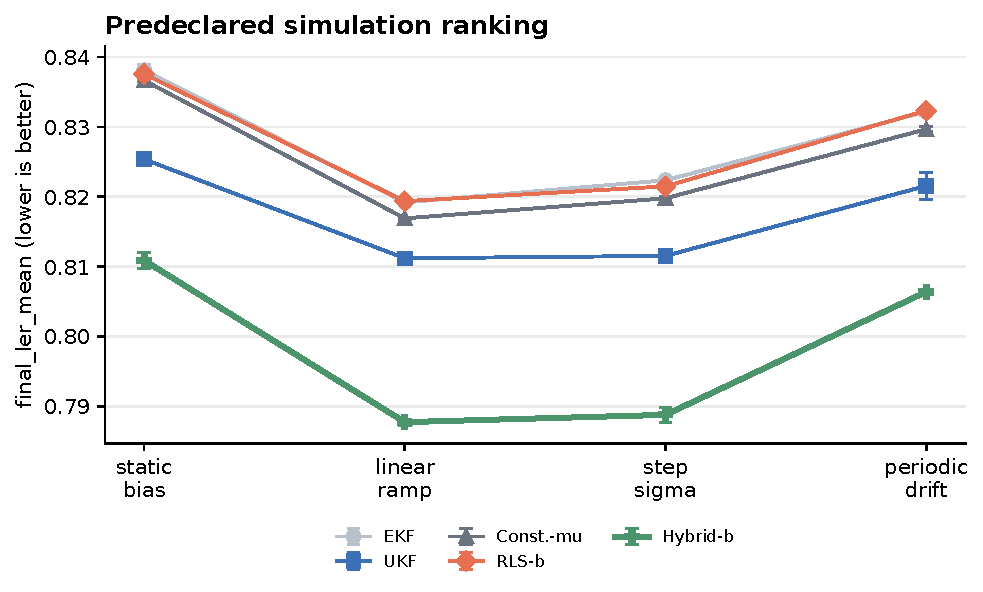
\includegraphics[width=0.95\linewidth]{fig02_main_software_hil_results.pdf}
\caption{Main \softwarehil{} comparison.  The plot visualizes the existing
\finalLER{} means from Table~\ref{tab:main-results}; lower is better.  Error
bars show descriptive standard deviations across the two available repeats
per scenario and mode.  The plot supports a predeclared four-scenario
\softwarehil{} ranking only.  Paired repeat deltas are provided in
Table~\ref{tab:paired-deltas}, the descriptive resampling envelope is provided
in Table~\ref{tab:paired-uncertainty}, and data-backed advantage
margins are provided in Table~\ref{tab:ler-advantage-margin}; all are bounded
by the accompanying supporting data.  Inferential confidence intervals, formal
hypothesis tests and unseen drift families remain open validation requirements.}
\label{fig:main-results}
\end{figure}

\subsection{Controlled nearest-syndrome, oracle and wrapped-Gaussian checks separate estimator and decoder limits}

These controlled baselines answer a narrow technical question: whether the
affine form is obviously dominated by a hard nearest-syndrome correction or a
known-state wrapped posterior rule in a local one-step setting.  They are
sanity checks for the fast-path approximation, not substitutes for a formal
known-noise or nearest-lattice benchmark.

To isolate whether the affine fast path is limited by the affine form itself,
by the upstream estimator or by the absence of a posterior branch model, we
added a small controlled local-Gaussian analysis.
The analysis samples 120,000 one-step errors for four representative drift
states, compares a hard nearest-syndrome correction, a fixed nominal affine
rule and an oracle affine rule that is given the state
\((\sigma,\mu_q,\mu_p,\vartheta)\), and adds one-step wrapped-Gaussian
posterior-mean and MAP branch baselines.

The result is deliberately narrower than the main benchmark.  The oracle
affine rule reduces residual MSE relative to the fixed nominal affine rule in
all four controlled states, with the largest reduction in the post-step state
(Table~\ref{tab:controlled-oracle-affine}).  The nearest-syndrome row is much
weaker in residual MSE because it applies the noisy wrapped syndrome directly
as a hard correction, making measurement noise and branch ambiguity visible.
The wrapped-Gaussian posterior mean is slightly better than oracle affine only
in the static state; in the ramp, step and periodic states it has higher MSE,
and the MAP branch rule is weaker still.  This mixed outcome is important.  It
shows that known-state affine correction captures a real local modelling
advantage, while a nearest-syndrome or wrapped-posterior comparator cannot be
treated as solved by simply adding a hard branch or branch prior to the
one-step setting.  A fully tuned sequence-level wrapped or nearest-lattice
baseline, a holdout drift set and \finalLER{}-level scoring remain required
before making stronger decoder-comparison claims.

\begin{table}[t]
\centering
\scriptsize
\setlength{\tabcolsep}{3pt}
\resizebox{\linewidth}{!}{%
\begin{tabular}{@{}lrrrrr@{}}
\toprule
Controlled state & Nearest syndrome & Fixed affine & Oracle affine & Wrapped mean & Wrapped MAP \\
\midrule
\texttt{static\_bias\_theta} & 0.232823 & 0.049199 & 0.048095 & \textbf{0.047955} & 0.048203 \\
\texttt{linear\_ramp\_midpoint} & 0.230689 & 0.061417 & \textbf{0.060251} & 0.062341 & 0.063105 \\
\texttt{step\_after\_jump} & 0.233626 & 0.108216 & \textbf{0.092541} & 0.105815 & 0.110339 \\
\texttt{periodic\_high\_phase} & 0.231307 & 0.081757 & \textbf{0.076028} & 0.082349 & 0.084002 \\
\bottomrule
\end{tabular}
}
\caption{Controlled local-Gaussian nearest-syndrome, oracle-affine and
wrapped-Gaussian checks.  Entries are one-step residual MSE; lower is better.
The nearest-syndrome row applies the wrapped syndrome directly as a hard
correction and is included as a one-step nearest-lattice-style sanity
reference, not as a tuned finite-energy nearest-lattice decoder.  The table
uses the manuscript affine mapper for the affine rows and known-state
wrapped-Gaussian posterior rules for the posterior rows.  It is a sanity check
for estimator and decoder limits, not a formal \softwarehil{} benchmark,
sequence-level wrapped decoder comparison, holdout-drift test or hardware
measurement.}
\label{tab:controlled-oracle-affine}
\end{table}

\subsection{A residual-boundary channel surrogate clarifies what \finalLER{} does and does not measure}

The half-lattice crossing rule can be written in channel language without
claiming a full logical-channel reconstruction.  For each controlled
local-Gaussian state, we decomposed residual boundary events into q-only,
p-only, simultaneous q/p and no-crossing outcomes.  This gives a
Pauli-channel-style surrogate
\[
    p_I^{\mathrm{surr}}=1-p_{\mathrm{any}},\quad
    p_{q}^{\mathrm{surr}},\quad p_{p}^{\mathrm{surr}},\quad
    p_{qp}^{\mathrm{surr}},
\]
where \(p_{\mathrm{any}}\) is the probability that the residual crosses at
least one half-lattice boundary.  If this decomposition is treated only as a
qubit Pauli-channel surrogate, it induces
\(F_{\mathrm{avg}}^{\mathrm{surr}}=(1+2p_I^{\mathrm{surr}})/3\).  The
manuscript does not use this quantity as a finite-energy GKP logical-channel
fidelity; it is included in the supporting data only to make the relationship
between residual-boundary scoring and fidelity language explicit.
The point of the table is therefore preventive as much as comparative: it
shows exactly where the protocol-defined LER proxy stops and where a genuine
finite-energy channel analysis would have to begin.

Table~\ref{tab:logical-channel-surrogate} reports the safer quantity,
\(p_{\mathrm{any}}\).  This union rate is related to, but not identical with,
the manuscript \finalLER{} definition: \finalLER{} counts q- and p-boundary
crossings separately, so a simultaneous q/p event contributes twice, whereas
\(p_{\mathrm{any}}\) asks whether at least one Pauli-like residual-boundary
event occurred in the sample.  The static and ramp states have no observed
affine crossings in 120,000 controlled samples, whereas the post-step and
periodic states expose low but nonzero residual-boundary events.  The
wrapped-Gaussian MAP branch rule has higher surrogate crossing probability in
all four states, again showing that branch-aware posterior logic needs a
tuned sequence-level protocol before it can serve as a stronger comparator.
The table supports only a residual-boundary event decomposition; it does not
estimate leakage, finite-energy envelopes, auxiliary-state noise, correlated
rounds or process fidelity.

\begin{table}[t]
\centering
\small
\begin{tabular}{@{}lrrrr@{}}
\toprule
Controlled state & Fixed affine & Oracle affine & Wrapped mean & Wrapped MAP \\
\midrule
\texttt{static\_bias\_theta} & 0.000000 & 0.000000 & 0.000000 & 0.000017 \\
\texttt{linear\_ramp\_midpoint} & 0.000000 & 0.000000 & 0.000042 & 0.000183 \\
\texttt{step\_after\_jump} & 0.000467 & 0.000467 & 0.002417 & 0.006450 \\
\texttt{periodic\_high\_phase} & 0.000042 & 0.000042 & 0.000617 & 0.001867 \\
\bottomrule
\end{tabular}
\caption{Residual-boundary Pauli-channel-style surrogate for the controlled
local-Gaussian states.  Entries are \(p_{\mathrm{any}}\), the probability of
at least one q/p half-lattice residual crossing; lower is better.  The source
CSV also records q-only, p-only, simultaneous crossing and
\(F_{\mathrm{avg}}^{\mathrm{surr}}\) fields, but the table reports only the
crossing probability to avoid presenting the surrogate as finite-energy
logical-channel tomography or process fidelity.}
\label{tab:logical-channel-surrogate}
\end{table}

\begin{table}[t]
\centering
\small
\begin{tabular}{@{}lrrrr@{}}
\toprule
Controlled state & Fixed affine & Oracle affine & Wrapped mean & Wrapped MAP \\
\midrule
\texttt{static\_bias\_theta} & 1.000000 & 1.000000 & 1.000000 & 0.999989 \\
\texttt{linear\_ramp\_midpoint} & 1.000000 & 1.000000 & 0.999972 & 0.999878 \\
\texttt{step\_after\_jump} & 0.999689 & 0.999689 & 0.998389 & 0.995700 \\
\texttt{periodic\_high\_phase} & 0.999972 & 0.999972 & 0.999589 & 0.998756 \\
\bottomrule
\end{tabular}
\caption{Pauli-style identity-surrogate readout derived from the same
residual-boundary event decomposition as Table~\ref{tab:logical-channel-surrogate}.
Entries are \(F_{\mathrm{avg}}^{\mathrm{surr}}=(1+2p_I^{\mathrm{surr}})/3\),
with \(p_I^{\mathrm{surr}}=1-p_{\mathrm{any}}\).  The table is included only
to make the manuscript's channel-language bridge traceable to supporting data;
it is not a finite-energy GKP logical-channel fidelity, process fidelity,
hardware fidelity or outer-code logical-error estimate.}
\label{tab:logical-channel-fidelity-surrogate}
\end{table}

The same supporting data can also be read at the method level
(Table~\ref{tab:lattice-logical-channel-sanity}).  This aggregation is useful
because it separates the question ``which method has the larger
residual-boundary channel surrogate?'' from the per-state event decomposition.
Across the four controlled local-Gaussian states, the fixed and oracle affine
rows have the lowest mean \(p_{\mathrm{any}}\), while the wrapped posterior MAP
row has the largest worst-state surrogate crossing rate.  This is still a
lattice-level residual-boundary sanity summary, not a finite-energy channel
measurement.

\begin{table}[t]
\centering
\small
\begin{tabular}{@{}lrlrrr@{}}
\toprule
Method & Mean \(p_{\mathrm{any}}\) & Worst state & Worst \(p_{\mathrm{any}}\) & Mean \(F_{\mathrm{avg}}^{\mathrm{surr}}\) & Worst \(F_{\mathrm{avg}}^{\mathrm{surr}}\) \\
\midrule
Fixed affine & 0.000127 & \texttt{step\_after\_jump} & 0.000467 & 0.999915 & 0.999689 \\
Oracle affine & 0.000127 & \texttt{step\_after\_jump} & 0.000467 & 0.999915 & 0.999689 \\
Wrapped mean & 0.000769 & \texttt{step\_after\_jump} & 0.002417 & 0.999488 & 0.998389 \\
Wrapped MAP & 0.002129 & \texttt{step\_after\_jump} & 0.006450 & 0.998581 & 0.995700 \\
\bottomrule
\end{tabular}
\caption{Method-level lattice sanity summary for the residual-boundary channel
surrogate.  Values aggregate the same controlled local-Gaussian states and
source rows as Tables~\ref{tab:logical-channel-surrogate}
and~\ref{tab:logical-channel-fidelity-surrogate}.  The table is included to
make the channel-language diagnostic easier to check; it is not finite-energy GKP
logical-channel fidelity, process tomography, hardware fidelity or an
outer-code logical-error estimate.}
\label{tab:lattice-logical-channel-sanity}
\end{table}

To move one step closer to finite-energy channel language without claiming
tomography, we also ran a simplified finite-squeezing measurement-channel
sanity check.  This check samples the same controlled drift states as the
residual-boundary analysis, adds a scalar finite-squeezing term \(\Delta\) and
an effective measurement-efficiency contribution to the wrapped syndrome, and
then compares three correction rules: hard nearest-syndrome correction, the
fixed affine fast path and an oracle affine rule.  The largest toy-channel
stress appears at \(\Delta=0.34\), where hard nearest-syndrome correction has a
mean \(p_{\mathrm{any}}\) of \(1.002\times10^{-3}\), while the fixed affine row
remains at \(1.625\times10^{-4}\) in the same toy model
(Table~\ref{tab:finite-energy-channel-sanity}).  This is useful as a
model-consistency check because it exercises the same half-lattice decision
surface after adding an explicit finite-squeezing noise scale.  It is still not
a calibrated finite-energy GKP logical-channel simulation, process fidelity
estimate or hardware result.

\begin{table}[t]
\centering
\small
\begin{tabular}{@{}llrlrr@{}}
\toprule
\(\Delta\) & Method & Mean \(p_{\mathrm{any}}\) & Worst state & Worst \(p_{\mathrm{any}}\) & Mean \(F_{\mathrm{avg}}^{\mathrm{surr}}\) \\
\midrule
0.18 & Hard nearest-syndrome & 0.000148 & \texttt{step\_after\_jump} & 0.000517 & 0.999901 \\
0.18 & Fixed affine & 0.000148 & \texttt{step\_after\_jump} & 0.000517 & 0.999901 \\
0.18 & Oracle affine & 0.000148 & \texttt{step\_after\_jump} & 0.000517 & 0.999901 \\
0.26 & Hard nearest-syndrome & 0.000160 & \texttt{step\_after\_jump} & 0.000475 & 0.999893 \\
0.26 & Fixed affine & 0.000129 & \texttt{step\_after\_jump} & 0.000458 & 0.999914 \\
0.26 & Oracle affine & 0.000129 & \texttt{step\_after\_jump} & 0.000458 & 0.999914 \\
0.34 & Hard nearest-syndrome & 0.001002 & \texttt{step\_after\_jump} & 0.001500 & 0.999332 \\
0.34 & Fixed affine & 0.000163 & \texttt{step\_after\_jump} & 0.000617 & 0.999892 \\
0.34 & Oracle affine & 0.000165 & \texttt{step\_after\_jump} & 0.000625 & 0.999890 \\
\bottomrule
\end{tabular}
\caption{Finite-squeezing toy-channel sanity check.  The table adds a scalar
finite-squeezing width \(\Delta\) to a simplified noisy wrapped-syndrome
measurement channel and reports residual half-lattice event probabilities for
three correction rules.  It is a toy measurement-channel consistency check
only, not a calibrated finite-energy GKP logical-channel fidelity estimate,
process tomography, formal benchmark, hardware fidelity or FPGA validation.}
\label{tab:finite-energy-channel-sanity}
\end{table}

\subsection{Sequence-level controlled baselines expose posterior-branch risk under drift}

We next repeated the nearest-syndrome, oracle and wrapped-Gaussian comparison over short drift
sequences rather than isolated samples.  Each scenario used 384 independent
sequences of 512 steps, the same local-Gaussian state families as the main
controlled analysis, and the same half-lattice residual-boundary proxy used in
the manuscript metric.  The sequence result preserves the one-step conclusion
that known-state oracle affine lowers residual MSE relative to a fixed nominal
affine rule, while the direct nearest-syndrome reference gives higher crossing
proxies in all four scenarios.  It also exposes a practical risk of
posterior-branch rules: the wrapped-Gaussian posterior mean and MAP references
produced higher sequence-level crossing proxies in the ramp, step and periodic states
(Table~\ref{tab:sequence-controlled-baselines}).

This result does not establish that affine decoding is globally superior to
wrapped decoding.  It shows that a branch-aware posterior comparator must be
implemented and tuned as a sequence-level decoder, not inserted as a naive
one-step branch rule.  The same caution applies to nearest-lattice-style
references: the present hard nearest-syndrome row is a stress reference, not a
formal nearest-lattice decoder.  For this manuscript, the result strengthens
the engineering rationale for a calibrated affine fast path while keeping the
stronger-baseline requirement open.

\begin{table}[t]
\centering
\small
\begin{tabular}{@{}lrrrrr@{}}
\toprule
Scenario & Nearest syndrome & Fixed affine & Oracle affine & Wrapped mean & Wrapped MAP \\
\midrule
\texttt{static\_bias\_theta} & 0.000214 & 0.000000 & 0.000000 & 0.000000 & 0.000000 \\
\texttt{linear\_ramp} & 0.000264 & 0.000015 & 0.000015 & 0.000158 & 0.000575 \\
\texttt{step\_sigma\_theta} & 0.000580 & 0.000310 & 0.000310 & 0.001221 & 0.003220 \\
\texttt{periodic\_drift} & 0.000229 & 0.000005 & 0.000005 & 0.000127 & 0.000519 \\
\bottomrule
\end{tabular}
\caption{Sequence-level controlled baseline analysis.  Entries are mean
half-lattice residual-boundary crossing proxies across 384 sequences of 512
steps; lower is better.  The nearest-syndrome row is a direct hard-correction
reference rather than a tuned nearest-lattice decoder.  This is a controlled
local-Gaussian sequence analysis, not the formal \softwarehil{} benchmark, a
confidence-interval run, a holdout drift test or hardware validation.}
\label{tab:sequence-controlled-baselines}
\end{table}

\subsection{Holdout drift stress tests expose adaptation space and lag sensitivity}

We next tested three drift patterns that were not part of the main
four-scenario comparison: a clipped random walk in the effective noise state,
two burst/reset intervals, and an oscillatory drift faster than the slow-loop
commit window.  The analysis used the same local-Gaussian displacement model
and the same 384-by-512 sequence shape as the controlled sequence study.  It
compared a fixed nominal affine rule, an oracle affine rule, a lagged-affine
reference with a 64-step commit interval and a 32-step lag, and the same
one-step wrapped-Gaussian posterior references.

The holdout stress test is informative because the half-lattice crossing proxy
is rare in these controlled samples.  The affine rows have the same observed
crossing rate within each holdout scenario, so residual MSE is the more
sensitive stress-test statistic.  The same supporting data also report a
residual-boundary Pauli-style identity surrogate; the oracle-affine
values remain near unity because crossings are rare, but this is still not a
finite-energy logical-channel fidelity.  Oracle affine gives the lowest
residual MSE in all three holdout families
(Table~\ref{tab:holdout-drift-stress}), showing that a correctly updated
affine surface still has adaptation headroom outside the main drift set.  The
lagged-affine row is deliberately mixed: it approaches oracle behavior under
random-walk drift, but it is worse than the fixed rule under burst/reset and
faster-than-window oscillation.  This failure mode is a useful constraint on
the method.  It indicates that the affine fast path is not the limiting idea
by itself; stale parameter commits can erase the adaptation benefit under
rapid or discontinuous drift.

The result does not prove generalization of the trained residual branch,
because the lagged row is a known-state slow-commit reference rather than the
CNN calibration module.  It also does not provide confidence intervals or a
formal expanded benchmark.  Its role is narrower: it adds an unseen-drift
stress layer that makes the proposed fast-path contract more falsifiable and
turns drift-tracking latency into a measurable design variable.

\begin{table}[t]
\centering
\small
\resizebox{\linewidth}{!}{%
\begin{tabular}{@{}lrrrrrr@{}}
\toprule
Holdout stress family & Fixed affine & Lagged affine & Oracle affine & Wrapped mean & Wrapped MAP & Oracle \(F_{\mathrm{avg}}^{\mathrm{surr}}\) \\
\midrule
\texttt{random\_walk\_drift} & 0.078869 & 0.073867 & \textbf{0.072685} & 0.078740 & 0.080857 & 0.999915 \\
\texttt{burst\_reset\_drift} & 0.066865 & 0.068622 & \textbf{0.062144} & 0.065936 & 0.067789 & 0.999780 \\
\texttt{faster\_than\_window\_oscillation} & 0.068354 & 0.068890 & \textbf{0.063745} & 0.067485 & 0.068764 & 0.999969 \\
\bottomrule
\end{tabular}
}
\caption{Controlled known-state holdout drift stress diagnostic.  Entries are residual MSE
across 384 sequences of 512 steps unless otherwise stated; lower residual MSE
is better.  \(F_{\mathrm{avg}}^{\mathrm{surr}}\) is the Pauli-channel-style
surrogate induced by the oracle-affine residual-boundary identity rate, not a
finite-energy logical-channel fidelity.  The lagged-affine row uses
known-state affine parameters committed every 64 steps with a 32-step lag, and
is a slow-loop lag reference rather than the trained residual branch.  The
table is a non-hardware stress test for the affine contract, not a formal
expanded benchmark, confidence-interval analysis or process-fidelity
estimate.}
\label{tab:holdout-drift-stress}
\end{table}

The same diagnostics can be read as a local-validity check for the affine
approximation (Table~\ref{tab:affine-local-validity}).  The short-sequence
rows ask whether an oracle affine surface has residual-MSE headroom over a
fixed nominal surface, and whether a naive wrapped-Gaussian posterior mean
reduces the half-lattice crossing proxy.  The holdout rows ask the same MSE
headroom question under unseen drift families and add a stale-commit risk
term, measured as lagged-affine residual MSE minus oracle-affine residual MSE.
This view is intentionally diagnostic: it supports the claim that affine
calibration has a local validity regime and identifiable failure modes, while
leaving a formal nearest-lattice, known-noise or wrapped-decoder benchmark as a
required validation step.

\begin{table}[t]
\centering
\scriptsize
\resizebox{\linewidth}{!}{%
\begin{tabular}{@{}llrrrl@{}}
\toprule
Surface & Layer & Oracle MSE gain (\%) & Branch-risk delta & Lag-risk delta & Readout \\
\midrule
\texttt{static\_bias\_theta} & Short sequence & 2.05 & 0.000000 & -- & local affine not dominated \\
\texttt{linear\_ramp} & Short sequence & 3.40 & 0.000142 & -- & local affine headroom visible \\
\texttt{step\_sigma\_theta} & Short sequence & 10.00 & 0.000910 & -- & local affine headroom visible \\
\texttt{periodic\_drift} & Short sequence & 3.43 & 0.000122 & -- & local affine headroom visible \\
\texttt{random\_walk\_drift} & Holdout stress & 7.84 & 0.006055 & 0.001182 & local affine headroom visible \\
\texttt{burst\_reset\_drift} & Holdout stress & 7.06 & 0.003792 & 0.006478 & stale commit can erase gain \\
\texttt{faster\_than\_window\_oscillation} & Holdout stress & 6.74 & 0.003740 & 0.005144 & stale commit can erase gain \\
\bottomrule
\end{tabular}
}
\caption{Affine local-validity diagnostic derived from the controlled sequence
and holdout-stress CSVs.  Oracle MSE gain is
\((\mathrm{MSE}_{\mathrm{fixed}}-\mathrm{MSE}_{\mathrm{oracle}})/
\mathrm{MSE}_{\mathrm{fixed}}\).  For short-sequence rows, branch-risk delta is
the wrapped-posterior-mean crossing proxy minus the oracle-affine crossing
proxy.  For holdout-stress rows, branch-risk and lag-risk deltas are
residual-MSE differences relative to oracle affine.  The table is a derived
diagnostic for the local affine approximation, not a formal nearest-lattice,
known-noise or wrapped-decoder benchmark, not a confidence-interval analysis
and not hardware evidence.}
\label{tab:affine-local-validity}
\end{table}

\subsection{Commit-lag sweeps turn stale parameters into a design variable}

The fixed 32-step lag in Table~\ref{tab:holdout-drift-stress} is only one
point on a slow-loop design surface.  We therefore swept the commit lag over
\(0,8,16,32,64\) and \(128\) simulation steps while keeping the commit interval
fixed at 64 steps.  The sweep reuses the three holdout drift families and
shared sampled errors within each family, so it is a controlled stale-parameter
diagnostic rather than a new benchmark.

The resulting pattern is deliberately not over-simplified
(Table~\ref{tab:commit-lag-sweep}).  Under random-walk drift, longer lag
monotonically increases residual MSE while still remaining below the fixed
nominal affine reference.  Under burst/reset and faster-than-window drift, the
lag surface is non-monotone because the stale state can occasionally land
closer to a later reset or oscillation phase than a recently committed state.
This is precisely why commit latency should be measured rather than inferred:
the fast affine surface remains cheap, but the slow-loop commit policy is part
of the method's empirical contract.

\begin{table}[t]
\centering
\small
\resizebox{\linewidth}{!}{%
\begin{tabular}{@{}lrrrrrr@{}}
\toprule
Holdout stress family & Lag 0 & Lag 8 & Lag 16 & Lag 32 & Lag 64 & Lag 128 \\
\midrule
\texttt{random\_walk\_drift} & 0.073831 & 0.073976 & 0.074130 & 0.074410 & 0.075173 & 0.076093 \\
\texttt{burst\_reset\_drift} & 0.067454 & 0.068193 & 0.068657 & 0.068694 & 0.068583 & 0.066913 \\
\texttt{faster\_than\_window\_oscillation} & 0.069251 & 0.069406 & 0.068989 & 0.069039 & 0.068842 & 0.068249 \\
\bottomrule
\end{tabular}
}
\caption{Commit-lag sweep for the lagged affine reference.  Entries are
residual MSE across 384 sequences of 512 steps; lower is better.  The commit
interval is fixed at 64 simulation steps and the columns sweep additional
simulation-step lag.  This table is a non-hardware stale-parameter diagnostic,
not a measured FPGA-latency result, source-vs-board agreement,
trained-branch holdout generalization, a confidence-interval analysis or
logical-channel fidelity.}
\label{tab:commit-lag-sweep}
\end{table}

\subsection{Analytical operation counts quantify the fast-path cost argument}

The cost advantage of the affine fast path is an analytical datapath argument,
not a measured FPGA-timing result.  The count assumes a two-quadrature
syndrome input, a \(2\times 2\) affine matrix, one bias vector, a single active
parameter bank and one correction per fast-loop shot.  It counts arithmetic and
small-state storage on the latency-critical path, while excluding the slow-loop
estimator, memory-controller implementation details and clock-frequency
closure.  Under this model, the affine rule uses one branch, four
multiplications, four additions and no exponential or division operations
(Table~\ref{tab:fast-path-cost-model}).  A 3-by-3 wrapped-Gaussian MAP
reference increases the multiplication count by 12.25-fold and the stored
state by 5.5-fold, while a posterior-mean reference requires softmax-like
nonlinear operations in addition to a larger arithmetic footprint.  This
comparison supports the design choice to keep posterior or learned estimation
outside the latency-critical correction path.  The cost model is a
candidate-selection argument for the hardware path, not a hardware
measurement.  It does not claim timing closure, resource use, power or
source-vs-board agreement.  Together with
the fixed-point and runtime-counter checks below, it provides the software
evidence available for the datapath contract in
Table~\ref{tab:fpga-datapath-contract}.

\begin{table}[t]
\centering
\small
\begin{tabular}{@{}>{\raggedright\arraybackslash}p{0.34\linewidth}rrrrr@{}}
\toprule
Decoder path & Branches & Mult. & Add. & Nonlinear ops & State scalars \\
\midrule
Affine fast path & 1 & 4 & 4 & 0 & 6 \\
Wrapped MAP, 3x3 branches & 9 & 49 & 40 & 0 & 33 \\
Wrapped posterior mean, 3x3 branches & 9 & 99 & 98 & 18 & 33 \\
\bottomrule
\end{tabular}
\caption{Analytical per-shot operation-count model.  The affine row counts the
two-quadrature matrix-vector correction used in the manuscript fast path.  The
wrapped rows count one-step known-state 3-by-3 branch references.  The table
supports a low-complexity design rationale only; it is not FPGA synthesis,
timing closure, power/resource measurement or hardware validation.}
\label{tab:fast-path-cost-model}
\end{table}

\subsection{Software fixed-point emulation bounds numerical degradation}

The affine fast path is intended to be representable as fixed-point arithmetic,
so the manuscript also checks numerical degradation before any board claim is
made.  We compared the floating-point affine runtime with the same runtime under
Q4.20 fixed-point emulation on 80,000 controlled local-Gaussian samples per
state.  The largest correction difference was \(1.6\times 10^{-6}\), no
scenario changed the residual-boundary crossing rate, and no fixed-point
quantization saturation occurred (Table~\ref{tab:fixed-point-parity}).  This
supports the fixed-point feasibility of the affine datapath under the tested
parameter range.  It does not establish board timing, source-vs-board agreement,
resource use or power.

\begin{table}[t]
\centering
\small
\begin{tabular}{@{}lrrrrr@{}}
\toprule
Scenario & Max diff & p99 diff & MSE delta & Crossing delta & Quant. sat. \\
\midrule
\texttt{static\_bias\_theta} & 0.000001 & 0.000001 & 0.000000 & 0.000000 & 0.000000 \\
\texttt{linear\_ramp\_midpoint} & 0.000001 & 0.000001 & 0.000000 & 0.000000 & 0.000000 \\
\texttt{step\_after\_jump} & 0.000002 & 0.000001 & 0.000000 & 0.000000 & 0.000000 \\
\texttt{periodic\_high\_phase} & 0.000001 & 0.000001 & 0.000000 & 0.000000 & 0.000000 \\
\bottomrule
\end{tabular}
\caption{Software fixed-point parity check for the affine fast path.  Entries
compare Q4.20 fixed-point emulation against the floating-point runtime under a
controlled local-Gaussian sample set.  Max and p99 diff are absolute correction
differences.  MSE delta and crossing delta are fixed-point minus floating-point.
This table is a numerical-emulation check only, not FPGA synthesis, timing
closure, source-vs-board agreement or hardware validation.}
\label{tab:fixed-point-parity}
\end{table}

\subsection{Runtime counters make the software contract observable}

The same \softwarehil{} comparison records runtime counters for commit activity,
cycle violations, overflow and saturation.  These counters do not measure board
latency or hardware reliability, but they make the stage-and-commit contract
observable in the software protocol.  Across the scenario-level comparison rows,
each mode applied about \(900\) commits on average, slow-update violations were
zero, correction saturation was zero, and the observed overflow rate was
approximately \(2.5\times10^{-3}\), dominated by histogram-input saturation
(Table~\ref{tab:runtime-discipline}).  This result supports the narrower claim
that the runtime contract exposes measurable software counters; it does not
establish board commit timing, rollback reliability or source-vs-board
agreement.

\begin{table}[t]
\centering
\small
\begin{tabular}{@{}>{\raggedright\arraybackslash}p{0.28\linewidth}rrrrr@{}}
\toprule
Mode & Commits & Slow viol. & Fast viol. & Overflow & Corr. sat. \\
\midrule
Constant Residual-Mu & 899.8 & 0 & 0.0000158 & 0.002582 & 0 \\
EKF & 899.8 & 0 & 0.0000158 & 0.002559 & 0 \\
Hybrid Residual-B & 899.9 & 0 & 0.0000158 & 0.002536 & 0 \\
RLS Residual-B & 899.8 & 0 & 0.0000158 & 0.002538 & 0 \\
UKF & 899.8 & 0 & 0.0000158 & 0.002571 & 0 \\
\bottomrule
\end{tabular}
\caption{Controlled-simulation runtime-discipline counters averaged across scenario-level
comparison rows.  The table reports controlled-simulation commit counts,
slow-update violation rate, fast-cycle violation rate, overflow rate and
correction-saturation rate.  It supports software observability of the
stage-and-commit contract only; it is not board commit latency, hardware
reliability or FPGA timing evidence.}
\label{tab:runtime-discipline}
\end{table}

\begin{figure}[t]
\centering
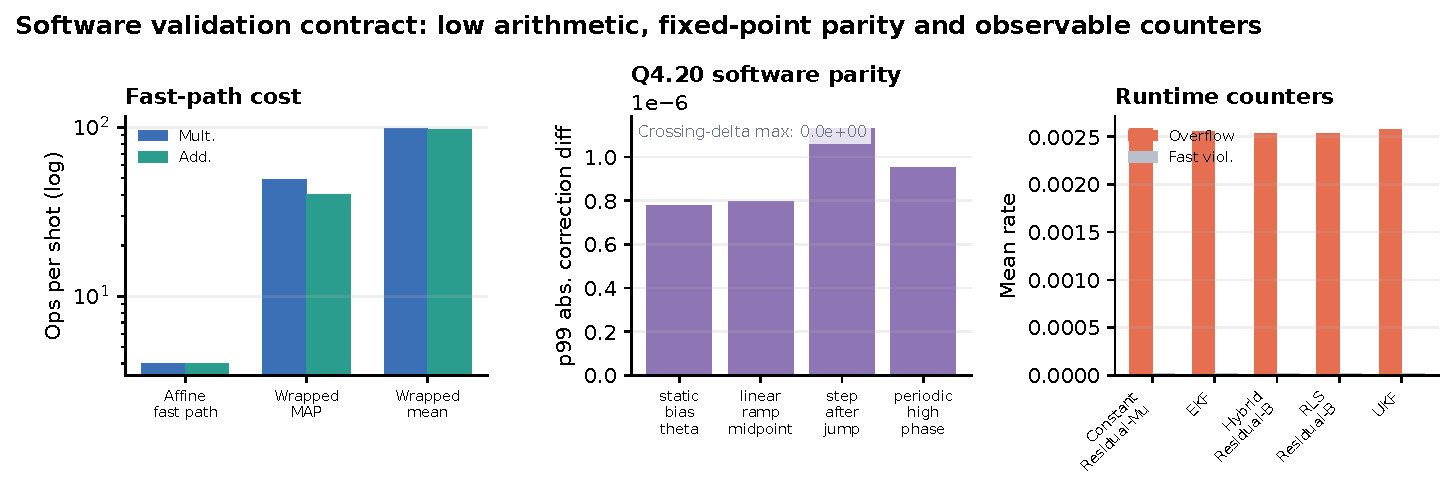
\includegraphics[width=0.98\linewidth]{fig05_validation_contract.pdf}
\caption{Software validation contract for the affine fast path.  Left:
analytical multiplication and addition counts compare the affine rule with
one-step wrapped-Gaussian references.  Middle: Q4.20 software fixed-point
emulation shows small p99 correction differences and no observed
residual-boundary crossing-rate change in the controlled sample set.  Right:
controlled-simulation runtime counters make overflow and fast-cycle violations
visible under the reported protocol.  The figure summarizes data-backed
software checks; it is not FPGA synthesis, timing closure, power/resource
measurement, source-vs-board agreement or board commit latency evidence.}
\label{fig:validation-contract}
\end{figure}

\subsection{Feature ablations constrain the mechanism story}

The feature and teacher ablation table shows that input choices materially
change performance in the tested scenario set (Table~\ref{tab:ablation}).  Removing
histogram deltas degrades performance relative to the full hybrid model,
which supports the use of recent histogram dynamics.  However, the
no-teacher-parameters row has the best four-scenario average.  The result
therefore does not support a simple claim that teacher parameters are
necessary or always beneficial.  It supports a weaker but more credible
interpretation: the residual calibration design is sensitive to feature
composition, and the mechanism evidence remains descriptive.

\begin{table}[t]
\centering
\small
\begin{tabular}{@{}lrrr@{}}
\toprule
Mode & Avg. LER & \(\Delta\) vs UKF & \(\Delta\) vs full hybrid \\
\midrule
\texttt{ukf} & 0.817382 & 0.000000 & +0.018837 \\
\texttt{hybrid\_full} & 0.798545 & -0.018837 & 0.000000 \\
\texttt{hybrid\_no\_hist\_deltas} & 0.826723 & +0.009341 & +0.028178 \\
\texttt{hybrid\_no\_teacher\_prediction} & 0.807251 & -0.010131 & +0.008706 \\
\texttt{hybrid\_no\_teacher\_params} & \textbf{0.749621} & -0.067761 & -0.048924 \\
\texttt{hybrid\_no\_teacher\_deltas} & 0.800329 & -0.017053 & +0.001784 \\
\bottomrule
\end{tabular}
\caption{Scoped feature and teacher ablation.  Negative deltas indicate lower
LER than the reference.  These rows support feature sensitivity, not causal
teacher necessity.}
\label{tab:ablation}
\end{table}

\begin{figure}[t]
\centering
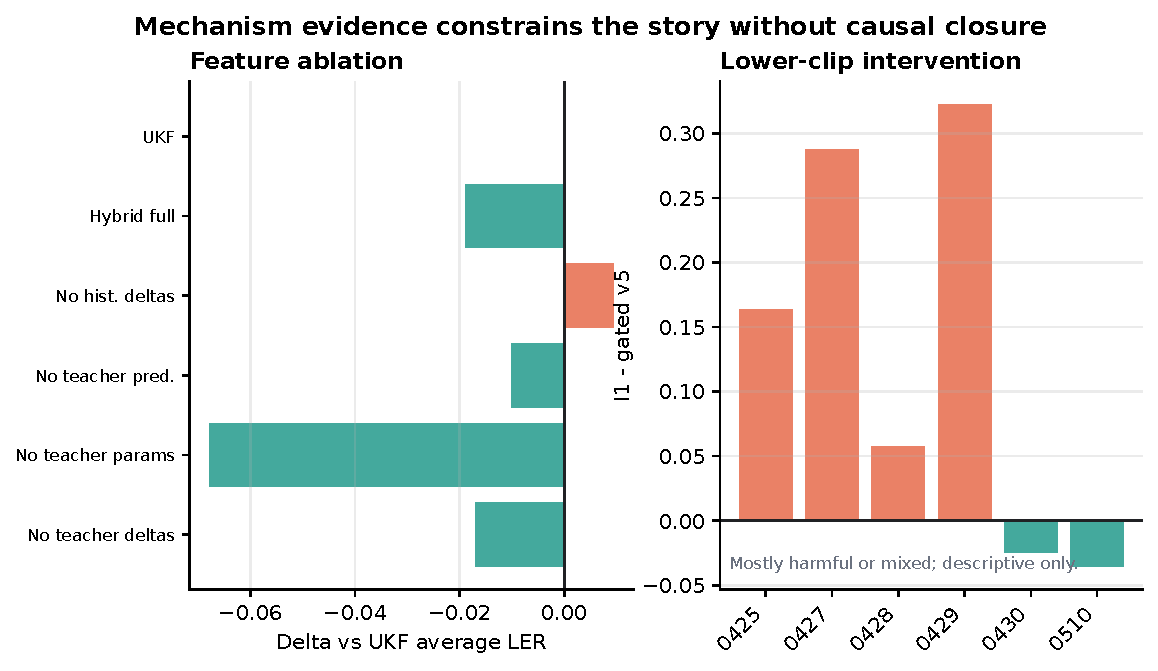
\includegraphics[width=0.95\linewidth]{fig03_ablation_and_mechanism.pdf}
\caption{Ablation and descriptive mechanism evidence.  Left: average LER
change relative to UKF for the scoped feature ablation table.  Right:
lower-clip intervention effect across the six-seed mechanism pack.  The
figure supports feature sensitivity and a cautionary intervention reading; it
does not establish a causal mechanism, teacher necessity or a successful
mitigation.}
\label{fig:ablation-mechanism}
\end{figure}

\subsection{Cross-seed intervention evidence remains descriptive}

The six-seed mechanism pack indicates that an instability pattern appears
across multiple seeds, but the tested lower-clip intervention is mixed and
mostly harmful (Table~\ref{tab:mechanism}).  This result is valuable because
it prevents an over-simple mechanism story.  Residual amplitude and committed
bias dynamics may participate in failures, but the reported intervention does
not show that lowering the residual clip is a general fix.

\begin{table}[t]
\centering
\small
\begin{tabular}{@{}lrrl@{}}
\toprule
Seed & Gated v5 -- Full & I1 -- Gated v5 & Verdict \\
\midrule
20260425 & 0.000907 & 0.163289 & harmful \\
20260427 & -0.145352 & 0.287166 & harmful \\
20260428 & -0.078998 & 0.057395 & harmful \\
20260429 & -0.127948 & 0.322245 & harmful \\
20260430 & -0.170777 & -0.024372 & mixed/no clear effect \\
20260510 & -0.003953 & -0.035533 & helpful \\
\bottomrule
\end{tabular}
\caption{Descriptive six-seed mechanism and intervention summary.  The
lower-clip intervention does not identify a causal mechanism and should not be
described as a mitigation.}
\label{tab:mechanism}
\end{table}

\subsection{Supplementary statistical calibration supports the contract}

The statistical-calibration rows are reported under a separate supplementary
protocol rather than under the predeclared main ranking protocol
(Table~\ref{tab:statcalib}).  They use the same affine runtime interface but
answer a different question: whether a non-neural estimator can populate the
committed \((K,b)\) surface at all.  They should therefore be read as
contract evidence, not as evidence that the neural branch was beaten in a fair
main-table comparison.  The absolute values in this extension are not
comparable to the main ranking because candidate generation and protocol
generation differ.  A fully matched comparator claim would require a single
predeclared protocol that fixes candidate generation, selection, repeats,
uncertainty handling and reporting before seeing the outcomes.

\begin{table}[t]
\centering
\small
\begin{tabular}{@{}lrrr@{}}
\toprule
Scenario & UKF & Hybrid-\(b\) & StatCalib extension (not matched) \\
\midrule
\texttt{static\_bias\_theta} & 0.825370 & 0.810902 & 0.431708 \\
\texttt{linear\_ramp} & 0.811201 & 0.787755 & 0.467083 \\
\texttt{step\_sigma\_theta} & 0.811548 & 0.788800 & 0.460016 \\
\texttt{periodic\_drift} & 0.821558 & 0.806392 & 0.438751 \\
\bottomrule
\end{tabular}
\caption{Supplementary statistical-calibration analysis.  The table documents
a separate estimator-protocol observation.  Because candidate generation and
selection are not matched to the main ranking protocol, these rows support the
generality of the affine interface but do not establish a fully matched
comparator, a unique clean threshold or a fair main-table ranking.  The
absolute values are not comparable to the main ranking because candidate
selection and protocol generation differ.}
\label{tab:statcalib}
\end{table}

\begin{figure}[t]
\centering
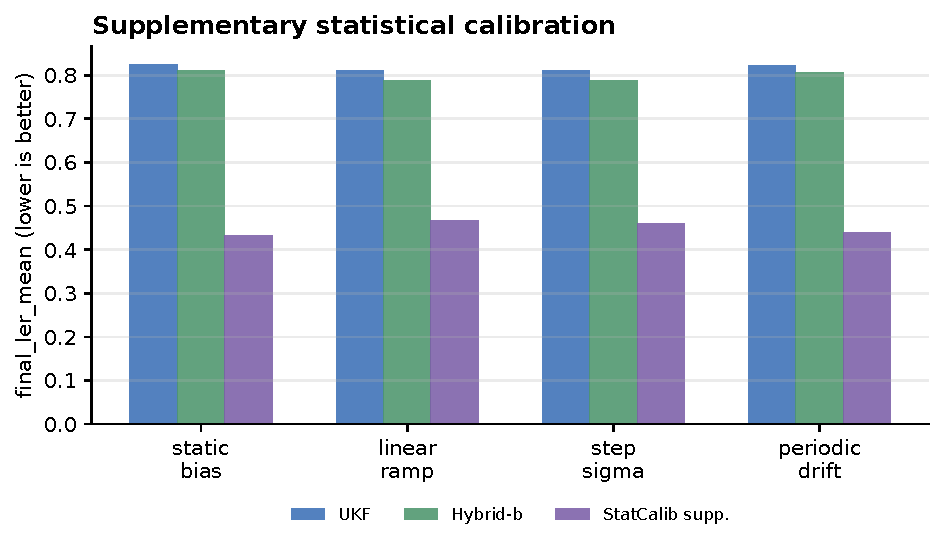
\includegraphics[width=0.95\linewidth]{fig04_statcalib_extension_lane.pdf}
\caption{Supplementary statistical-calibration analysis.  The plot compares
UKF, hybrid-\(b\) and the statistical-calibration values already listed in
Table~\ref{tab:statcalib}.  The result supports the broader affine calibration
contract, but it must remain separate from the main comparison because it was
not generated under the same predeclared ranking protocol; the absolute values
should not be interpreted as a matched win over the main hybrid branch.}
\label{fig:statcalib}
\end{figure}

\subsection{Required hardware and deployment measurements}

The present manuscript does not contain real-board execution results.  The
available deployment-adjacent material supports only one narrow runtime
statement: selected preserved \texttt{.tflite} files executed in an
isolated software runtime.  Board execution, timing, resource, power and
source-vs-board measurements are absent from this study.
Table~\ref{tab:hardware-plan} defines the hardware measurements required for an
implementation-stage evaluation.

\begin{table}[t]
\centering
\small
\begin{tabular}{@{}>{\raggedright\arraybackslash}p{0.28\linewidth}>{\raggedright\arraybackslash}p{0.28\linewidth}>{\raggedright\arraybackslash}p{0.34\linewidth}@{}}
\toprule
Hardware-facing item & Manuscript treatment & Evidence needed for hardware claims \\
\midrule
Board platform and host & \hardwareclaimrequired{} & Linux + FPGA host,
device path, permissions, board model and driver version. \\
\addlinespace
Bitstream / RTL / DMA interface & \hardwareclaimrequired{} & Bitstream hash,
AXI map, DMA histogram shape, element width and timeout policy. \\
\addlinespace
Fast-path latency & \hardwareclaimrequired{} & p50/p95/p99 and worst-case
cycles for \(Ks+b\), clipping and bank selection. \\
\addlinespace
Commit latency and reliability & \hardwareclaimrequired{} & stage, commit,
acknowledgement, rollback and stale-parameter counters. \\
\addlinespace
Resource and power & \hardwareclaimrequired{} & LUT/FF/DSP/BRAM, clock
frequency, timing closure and power. \\
\addlinespace
Source-vs-board agreement & \hardwareclaimrequired{} & fixed-point
agreement between software reference and board output on shared test vectors. \\
\bottomrule
\end{tabular}
\caption{Hardware-measurement requirements.  These entries define the
implementation-stage evidence required before hardware claims can be made;
they are not results of the present study.}
\label{tab:hardware-plan}
\end{table}

\section{Discussion}

The present results support a specific systems claim for drift-adaptive GKP
decoding: nonstationary syndrome statistics can be converted into updates of a
physical-layer affine correction surface while the per-shot correction remains
deterministic.  The main evidence is the predeclared ranking of the hybrid
residual branch under a controlled \softwarehil{} protocol.  Scoped ablations
and the supplementary statistical-calibration analysis sharpen the
interpretation.  Teacher features, histogram dynamics and estimator choice
affect the result, but the object that persists across these variants is the
committed affine surface consumed by the fast path.  This places the work
between soft-information GKP decoding, which exploits analog syndrome
structure, and real-time hardware decoding, which requires bounded latency and
verifiable datapaths.  The distinctive design choice is the separation of
roles: the slow loop absorbs nonstationary statistics, while the correction
cycle evaluates only a small affine matrix-vector update.

The supplementary statistical-calibration analysis reinforces this reading from
the opposite direction.  If a simple non-neural estimator can be strong under
the same runtime contract, the scientific object is the contract itself:
recent syndrome statistics update a low-dimensional affine surface that the
fast path can consume safely.  The CNN branch is one useful slow-loop
estimator, not the only possible estimator and not a final comparator.

Several alternative explanations are therefore constrained, but not eliminated.
The paired rows and advantage-margin readout show that the UKF-versus-hybrid
direction is consistent in the available repeats, but the two-repeat design is
still too small for an all-scenario inferential statistical claim.  The
completed 12-paired-repeat \texttt{static\_bias\_theta} and
\texttt{linear\_ramp} checks are important scenario-level exceptions: both give
positive paired-\(t\) and bootstrap interval lower bounds for UKF-minus-hybrid
\finalLER{} deltas.  They do not, by themselves, justify pooled or
all-scenario significance language.  The ablation and
statistical-calibration results make a pure ``CNN wins because it is neural''
interpretation too strong: feature design, histogram dynamics and the affine
commit contract remain part of the effect.  The residual-boundary channel
surrogate also rules out a purely notational fidelity claim, because it states
exactly which q/p half-lattice crossing events are being counted and which
finite-energy channel quantities remain outside the analysis.  Finally, the oracle and
wrapped-Gaussian checks indicate that a local posterior-style rule is not an
automatic replacement for the affine contract under drift, while also showing
that stronger known-noise and sequence-level baselines remain necessary before
making a broad decoder-comparison claim.

The supported claim is therefore an interface-level design trade-off, grounded
in the falsification-oriented design logic of
Table~\ref{tab:falsification-design} and in three linked but
non-substitutable tests.  First, the software benchmark tests
whether recent syndrome statistics can improve the protocol-defined
\finalLER{} of a deterministic correction surface under drift.  Second, the
residual-boundary channel surrogate tests whether that same improvement can be
translated into q/p event language without upgrading it to finite-energy
logical-channel fidelity.  Third, the implementation-feasibility checks test
whether the online rule remains small enough to be a plausible real-time
datapath: latency is addressed structurally by placing estimation in the slow
loop and leaving the fast path as \(\Delta_t=K_t s_t+b_t\), while cost and
verifiability are supported by the analytical operation-count model,
fixed-point software parity and the small source-vs-board target implied by a
clipped affine datapath.  These points motivate hardware validation, but they
are not hardware results: board timing, resource use, power, commit
reliability and source-vs-board vectors remain to be measured.

The numerical scale of adjacent work clarifies the comparison rather than
changing the supported claim.  Drift-aware graph reweighting and decoder-prior
optimization have already shown that calibration can produce large gains:
DGR reports a \(3.6\times\) average mismatch-LER reduction and much larger
worst-case improvements under drifted correlated noise, while experimental
prior optimization reports \(48\%\), \(16\%\) and \(3.3\%\) LER improvements in
different calibrated-decoder settings \cite{dgr2023,sivak2024}.  These numbers
make calibration a serious comparator rather than a rhetorical motivation.
The distinction here is the calibrated object: instead of updating an
outer-code graph, prior table or full neural decoder state, the slow loop
commits a two-quadrature physical correction surface \((K,b)\).  Calibration-conditioned learned decoders report
large experimental data sets, up to 11.11-fold LER reduction on recalibrated
chains and folded-FiLM latencies of about \(85\)--\(95\,\mu\mathrm{s}\)
\cite{stein2026}; AI pre-decoders report sub-step runtimes such as
\(38.78\,\mu\mathrm{s}\) \cite{chamberland2026}.  Real-time hardware decoders
set a different standard: lookup-table decoders report \(28\)--\(42\) ns
online latency with compressed memory \cite{lilliput2022}, distributed FPGA
surface-code decoding has been reported at \(11.5\) ns per measurement round
\cite{helios2023}, and integrated neural FPGA decoding has reported a
\(550\) ns closed-loop path with \(124\) ns neural decoding in a 17-qubit
surface-code experiment \cite{yang2026}.  These values are not normalized
baselines for the present software study.  They define the external measurement
standard for the proposed affine fast path: a stronger hardware version of this
work must report board latency, resource and power, source-vs-board agreement
and commit reliability while preserving the scientific separation between
slow-loop adaptation and the per-shot affine correction.

This distinction is the main comparative trade-off of the present formulation.
Relative to analog GKP and surface-GKP decoders, the method does not attempt to
replace the outer-code likelihood engine.  It supplies a physical-layer
calibration surface whose state can be logged, clipped and committed.  Relative
to calibration-conditioned neural decoders, it does not place the learned model
on the per-shot path; the online computation remains a deterministic affine
correction even when the committed parameters were produced by a CNN, a teacher
anchor or a statistical estimator.  Relative to hardware-tailored FPGA decoders,
it does not report measured device latency, but it does provide a smaller
and more directly replayable target for source-vs-board validation.  The
present data therefore support an interface-level design trade-off rather than a
single universal advantage: controlled-drift adaptation is paired with a
bounded arithmetic footprint, fixed-point-checkable numerical behaviour and a
traceable parameter-bank contract, while measured hardware advantage remains
untested.  The same affine contract also separates the latency-area
trade-off from the estimator design: parallel multipliers and serialized
multipliers implement the same committed map and can be validated against the
same source trace.
The verification target is smaller for the same reason the online datapath is
smaller.  A board implementation would need to reproduce six affine parameters,
two clipped syndrome inputs, two correction outputs and a bounded set of status
flags at each shot boundary.  A per-shot neural or wrapped-posterior datapath
would also require validating hidden activations, branch scores or nonlinear
approximations.  The expected advantage is therefore not only fewer arithmetic
operations, but a narrower object for bit-accurate replay and failure analysis.
This reading also explains why the manuscript keeps four metrics side by side
instead of collapsing them into one score.  The \finalLER{} rows test whether
the affine surface reduces the protocol-defined error proxy under drift; the
residual-boundary surrogate prevents that proxy from being overstated as
finite-energy channel fidelity; the operation-count and fixed-point rows test
whether the online rule is small enough for a real-time datapath; and the
calibration rows test whether more than one estimator can populate the same
committed interface.  The joint claim is an interface-level one: adaptation,
cost and traceability improve together only because the fast path remains a
low-dimensional affine correction.

\begin{table}[t]
\centering
\small
\begin{tabular}{@{}>{\raggedright\arraybackslash}p{0.20\linewidth}>{\raggedright\arraybackslash}p{0.28\linewidth}>{\raggedright\arraybackslash}p{0.25\linewidth}>{\raggedright\arraybackslash}p{0.15\linewidth}@{}}
\toprule
Advantage dimension & Supported basis in this study & Relation to prior work & Required upgrade \\
\midrule
Latency-critical role &
The per-shot rule is a \(2\times2\) affine map plus clipping and bank selection;
the learned estimator is outside the per-shot path. &
Complements AI pre-decoders and calibration-conditioned learned decoders by
placing learning in a slow calibration loop rather than in the correction
datapath. &
Measured board latency distribution. \\
\addlinespace
Noise adaptation &
The hybrid branch ranks lowest by mean \finalLER{} in the four tested drift
scenarios; controlled stress tests expose random-walk, burst/reset and
faster-than-window regimes. &
Addresses a physical-layer GKP correction surface rather than only
outer-code graph weights, decoder priors or message-passing reliabilities. &
Repeat-expanded holdout benchmark. \\
\addlinespace
Calibration object &
The committed runtime state is the low-dimensional \((K,b)\) affine surface,
not a full per-shot neural decision rule or an outer-code edge-weight table. &
Keeps the adaptation target closer to the analog GKP displacement operation
than graph reweighting, prior optimization or calibration-conditioned neural
decoding. &
Matched device-derived calibration traces. \\
\addlinespace
Cost and verifiability &
The affine count is \(4\) multiplications, \(4\) additions and \(6\) stored
state scalars per shot, with Q4.20 software parity under controlled samples;
parallel or serialized multiplier schedules preserve the same source trace. &
Gives a smaller source-vs-board verification target than a branch-aware
posterior rule or a per-shot neural decoder. &
Synthesis, resource and power reports. \\
\addlinespace
GKP metric interpretation &
\finalLER{} counts q/p half-lattice boundary crossings, and the
residual-boundary surrogate decomposes the same events into channel-language
categories. &
Connects the protocol to approximate-GKP logical-boundary reasoning while
remaining narrower than finite-energy channel fidelity. &
Logical-channel reconstruction. \\
\addlinespace
Hardware extension path &
The manuscript specifies timing, commit, resource, power and source-vs-board
measurements needed for an FPGA demonstration. &
Uses real-time decoder literature as the measurement standard, not as evidence
for this implementation. &
Device logs, bitstream/RTL hash and board vectors. \\
\bottomrule
\end{tabular}
\caption{Supported design trade-off and the evidence needed to strengthen
each claim.  The table summarizes what is established by the present software
and analytical evidence, how that differs from adjacent GKP, learned-decoder and
real-time-decoder work, and what would be required before making stronger
hardware or channel-level claims.}
\label{tab:supported-advantage}
\end{table}

A successful FPGA experiment would therefore strengthen three specific physical
interface claims, rather than simply add a hardware label to the present
software result.  First, bit-accurate source-vs-board replay would show that
the committed \((K,b)\) banks define a reproducible physical displacement
surface.  Second, measured fast-path and commit latency would test whether
slow-loop adaptation can be kept outside the control-cycle boundary.  Third,
resource, power and fault-log measurements would test whether the small affine
state is cheaper to audit than a per-shot neural or posterior-branch datapath.
If those conditions are met, the main advantage over adjacent learned-decoder
and real-time-decoder work would be a measured separation of roles: richer
statistics or learned estimators may operate in the calibration layer, whereas
the latency-critical correction remains a deterministic physical displacement
rule.  Such a result would still not by itself prove a surface-code threshold,
finite-energy logical-channel fidelity or broad holdout robustness, but it
would convert the affine-contract argument into a tested real-time calibration
interface.

The scope of inference follows directly from this decomposition.  The drift
claim is strongest inside the predeclared four-scenario \softwarehil{} table
and the two completed 12-pair scenario checks.  The random-walk, burst/reset
and faster-than-window stress tests broaden the diagnostic picture, but they
use controlled known-state drift families rather than a trained-branch holdout
benchmark.  The nearest-syndrome, oracle-affine and wrapped-Gaussian checks
separate estimator error, hard-correction risk and local affine validity, but
they do not constitute a full nearest-lattice or sequence-level known-noise benchmark.
The residual-boundary surrogate gives channel-language bookkeeping for q/p
half-lattice crossings, not finite-energy logical-channel fidelity.

These limitations define the validation required for stronger claims.
Statistically, the descriptive paired envelope should be replaced by
repeat-expanded or inferential uncertainty estimates across all drift
scenarios.  Algorithmically, known-noise affine, nearest-lattice and
sequence-level wrapped-Gaussian baselines should be run under the same
predeclared protocol.  Physically, finite-energy logical-channel probabilities
or channel infidelity should be estimated under specified noise channels before
making fidelity-level claims.  For hardware, the decisive evidence would be
bit-accurate source-vs-board agreement, measured fast-path and commit latency,
synthesis/resource reports and power measurements.  Until those layers are
added, the manuscript supports a controlled-simulation quantum-engineering
systems method rather than a deployment result.

\section{Conclusion}

We presented a runtime-consistent affine calibration formulation for
drift-adaptive GKP decoding.  The method keeps the per-shot correction as the
small affine rule \(\Delta_t=K_t s_t+b_t\) while updating the affine
parameters from recent syndrome statistics in a slower loop.  Under a
predeclared four-scenario \softwarehil{} protocol, the main-table hybrid
residual branch has the lowest mean \finalLER{} in all tested scenarios.
The formal repeat-expanded evidence is narrower: 12-paired-repeat
\texttt{static\_bias\_theta} and \texttt{linear\_ramp} checks support positive
scenario-level UKF-minus-hybrid intervals, while the remaining scenarios still
require the same treatment before broad interval wording is justified.
Scoped ablations and mechanism materials support a conservative
interpretation: histogram dynamics and feature design matter, and the more
general object is the affine calibration interface rather than
teacher-parameter necessity.  Controlled
oracle-affine and wrapped-Gaussian checks show that known effective-state
affine parameters reduce residual MSE in local-Gaussian states, while a simple
wrapped posterior does not dominate in either one-step or short-sequence
settings.  A supplementary statistical-calibration analysis further supports
the affine-contract view, while remaining separate from the main comparison.

Together, these results define a controlled-simulation systems method for
drift-adaptive GKP correction.  The contribution is the combination of a
physical-layer calibration target, a deterministic low-cost fast path and a
metric hierarchy that separates LER proxy, channel-language surrogate, software
arithmetic and hardware-stage measurements.  The distinctive advantage,
relative to adjacent soft-information, learned-decoder and FPGA-decoder work,
is the separation of adaptation from the latency-critical correction: the slow
loop may use richer statistics or learned estimators, whereas the fast loop
remains a small affine displacement rule that can be quantized, replayed and
verified.  The present manuscript therefore establishes an interface-level
claim: adaptive GKP calibration can improve a controlled drift benchmark while
preserving a fast-path object suitable for fixed-point replay and later board
measurement.  Deployment-level and broad benchmark claims remain outside that
claim until measured device timing and resource use, independent runtime
portability, expanded drift coverage, stronger baselines and repeat-expanded
uncertainty estimates are available.

\section{Outlook}

The validation programme implied by these data has three axes.  First,
statistical benchmark expansion should add repeat-expanded uncertainty
estimates, trained-branch holdout drift families and formal known-noise affine,
nearest-lattice or sequence-level wrapped-Gaussian baselines under a
predeclared protocol.  Second, physics and channel validation should test the
lattice constant, syndrome wrap interval, logical boundary and \finalLER{}
definition before using finite-energy logical-channel simulations to support
channel-level fidelity claims.  Third, hardware validation should replace the
present interface specification with board data: device paths, bitstream or RTL
hashes, DMA or MMIO evidence, latency distributions, resource use, power,
commit reliability and source-vs-board numerical agreement.  These studies
would determine whether the affine calibration contract remains advantageous
beyond the present \softwarehil{} setting.

\appendix

\section*{Supplementary reporting overview}

The supplementary sections collect reporting details that make the manuscript
traceable without expanding the empirical claims made in the Results and
Discussion.  They specify the data classes, protocol definitions, terminology,
figure inputs and additional measurements needed before stronger statistical,
channel-level or hardware conclusions could be drawn.

\section{Supplementary Literature Metric Crosswalk}

The following tables record the representative external metrics used to orient
the related-work comparison in the main text.  They are comparison anchors, not
normalized baselines or results generated by this study.

\begin{table}[htbp]
\centering
\small
\begin{tabular}{@{}>{\raggedright\arraybackslash}p{0.19\linewidth}>{\raggedright\arraybackslash}p{0.30\linewidth}>{\raggedright\arraybackslash}p{0.35\linewidth}@{}}
\toprule
Comparison axis & Representative prior-work metrics & Relevance to this paper \\
\midrule
Analog GKP information &
Analog syndrome decoding has been reported to lower required squeezing from
about \(16.0\) dB to \(9.8\) dB in surface-GKP settings
\cite{fukui2018,noh2020}. &
The present work does not claim novelty in analog information.  It uses recent
analog histograms to update a low-dimensional affine correction surface. \\
\addlinespace
Calibration-aware QEC &
Prior calibration and drift-aware graph updates report gains ranging from
percentage-level prior improvements to multi-fold mismatch reductions
\cite{dgr2023,chen2022,sivak2024}. &
The calibrated object here is the physical-layer \((K,b)\) surface consumed by
the fast GKP correction path, not only an outer-code graph weight or decoder
prior. \\
\addlinespace
Logical-error and overhead targets &
Surface-GKP studies report logical-failure and overhead targets such as
\(0.87\%\) to \(0.36\%\) CNOT-failure reduction, \(9.9\) dB threshold behavior,
and \(291\) modes plus \(97\) qubits versus \(1457\) bare qubits for a matched
low-failure target \cite{noh2022}. &
The present metric is narrower: it is a protocol-defined q/p boundary-crossing
proxy, not the same endpoint as prior-work LER or logical-failure rates.  The
result should therefore be read as a front-end calibration result, not as an
end-to-end surface-GKP overhead claim. \\
\addlinespace
Logical-channel fidelity and infidelity &
Approximate-GKP analyses report logical-channel probabilities, loss-channel
infidelity and near-optimal loss/amplification performance as channel-level
figures of merit \cite{jafarzadeh2025,hastrup2023,zheng2024}. &
This manuscript reports a residual-boundary Pauli-channel-style
surrogate derived from q/p half-lattice crossings, but not finite-energy
logical-channel fidelity or process infidelity.  Fidelity-level claims would
require channel-specific simulation, logical-channel probability estimates or
process-infidelity reconstruction under a specified physical channel. \\
\bottomrule
\end{tabular}
\caption{External GKP and calibration comparison axes.  The cited values are
representative reported metrics from adjacent work, not normalized baselines
for this study.  They position the contribution and the validation required
without treating incompatible metrics as results of this manuscript.}
\label{tab:external-comparison}
\end{table}

\begin{table}[htbp]
\centering
\small
\begin{tabular}{@{}>{\raggedright\arraybackslash}p{0.19\linewidth}>{\raggedright\arraybackslash}p{0.30\linewidth}>{\raggedright\arraybackslash}p{0.35\linewidth}@{}}
\toprule
Comparison axis & Representative prior-work metrics & Relevance to this paper \\
\midrule
Real-device learned decoding &
Learned decoders have reported real-processor LER reductions using large
experimental and synthetic data sets \cite{bausch2024,stein2026}. &
The present manuscript does not report real-processor learned-decoder LER.  It
uses software drift scenarios to test whether a learned slow loop can populate
a deterministic affine surface. \\
\addlinespace
Structured neural and soft decoders &
Bosonic/GKP-like neural decoders, neural matching-weight predictors and
hardware soft-information decoders provide related routes to improved LER or
thresholds \cite{wang2022,peled2026,hanisch2026}. &
The present work does not claim novelty in neural decoding or soft information.
Its distinction is that the neural component is confined to slow calibration
of the affine physical correction surface. \\
\addlinespace
Runtime pre-decoders and calibration-conditioned latency &
AI pre-decoders and calibration-conditioned decoders report runtime anchors
such as \(38.78\,\mu\mathrm{s}\) sub-step decoding or \(85\)--\(95\,\mu\mathrm{s}\)
folded FiLM latency \cite{chamberland2026,stein2026}. &
The latency argument in this manuscript is analytical and software-emulated.  A
device study must measure the affine fast path directly rather than borrow these
per-shot neural latency values. \\
\addlinespace
Real-time FPGA decoders &
Hardware decoders report deployment metrics such as \(28\)--\(42\) ns lookup
latency and compressed lookup memory \cite{lilliput2022}, \(11.5\) ns per
measurement round \cite{helios2023}, sub-\(\mu\)s round or feedback timing
\cite{caune2024,ziad2024,maurer2025}, 550 ns closed-loop latency and
QPU-feedback integration \cite{yang2026}, and scale, memory, area and power
figures \cite{collision2025}. &
These works define the standard for hardware claims.  This manuscript only
specifies the required hardware measurement surface until the same classes of
timing, resource and source-vs-board data are available. \\
\bottomrule
\end{tabular}
\caption{External learned-decoder and hardware-runtime comparison axes.  The
cited values are representative reported metrics from adjacent work, not
normalized baselines for this study.  They position the slow-loop calibration
role and the required hardware validation, not as results of this manuscript.}
\label{tab:external-runtime-comparison}
\end{table}

\section{Data, Code, and Reproducibility Availability}

This appendix separates materials used by the present study from materials
required for broader statistical, deployment or hardware claims.  Available
analysis records support the controlled-simulation methods reported here, but
they do not by themselves establish a hardware demonstration, a deployment
study or a normalized broad-decoder leaderboard.

\begin{table}[htbp]
\centering
\scriptsize
\setlength{\tabcolsep}{4pt}
\begin{tabular}{@{}>{\raggedright\arraybackslash}p{0.26\linewidth}>{\raggedright\arraybackslash}p{0.30\linewidth}>{\raggedright\arraybackslash}p{0.30\linewidth}@{}}
\toprule
Material class & Material used in this manuscript & Interpretation limit \\
\midrule
Predeclared simulation results & Four-scenario, five-mode ranking used in
Table~\ref{tab:main-results}. & Supports relative ranking only inside the
predeclared simulation protocol. \\
\addlinespace
Ablation and mechanism materials & Feature and cross-seed intervention tables
used in Tables~\ref{tab:ablation} and~\ref{tab:mechanism}. & Descriptive
mechanism evidence; not a causal proof. \\
\addlinespace
Statistical-calibration extension & Supplement-side comparison in
Table~\ref{tab:statcalib}. & Supports the affine-calibration contract; does
not promote statistical calibration as a validated main comparator. \\
\addlinespace
Controlled nearest-syndrome, oracle and wrapped-Gaussian checks & One-step and
short-sequence local-Gaussian comparisons in
Tables~\ref{tab:controlled-oracle-affine}
and~\ref{tab:sequence-controlled-baselines}. & Supports estimator,
hard-correction and decoder-limit sanity checks only; does not replace formal
stronger baselines or \finalLER{} validation. \\
\addlinespace
Holdout drift stress tests & Random-walk, burst/reset and faster-than-window
controlled stress families in Table~\ref{tab:holdout-drift-stress}. & Supports
non-hardware unseen-drift diagnostics only; does not establish trained-branch
holdout generalization, confidence intervals or hardware robustness. \\
\addlinespace
Residual-boundary channel surrogate & q/p half-lattice crossing event
decomposition in Table~\ref{tab:logical-channel-surrogate} and method-level
lattice sanity summary in Table~\ref{tab:lattice-logical-channel-sanity}. &
Supports a Pauli-event surrogate bridge between residual-boundary scoring and
channel language only; does not estimate finite-energy logical-channel
fidelity, process fidelity or hardware fidelity. \\
\addlinespace
Fast-path cost model & Analytical operation-count comparison in
Table~\ref{tab:fast-path-cost-model}. & Supports low-complexity motivation
only; does not establish FPGA timing, power or resource use. \\
\addlinespace
Fixed-point parity check & Q4.20 software-emulation comparison in
Table~\ref{tab:fixed-point-parity}. & Supports numerical fixed-point
feasibility under controlled samples only; does not establish source-vs-board
agreement, synthesis, timing closure, resource use or power. \\
\addlinespace
Literature metric crosswalk & Cited metric anchors for the external comparison
table, including paper-level figure, table and equation anchors where
available. & Supports related-work positioning only; not a normalized
leaderboard and not experimental data generated by this study. \\
\addlinespace
Training and runtime support & A clean CPU-only rerun and selected isolated
\texttt{.tflite} runtime checks. & Does not establish full
reproducibility, default-environment portability or validated deployed
operation. \\
\addlinespace
Hardware validation requirements & Hardware measurement checklist without board
measurements. & Does not establish board execution, timing, resource or
source-vs-board agreement. \\
\bottomrule
\end{tabular}
\caption{Availability of supporting materials.  Each row states how a material
class is used in the manuscript and what stronger conclusion it cannot support.}
\label{tab:availability}
\end{table}

For a stronger empirical version of the study, the supporting material should
include machine-readable result tables with seeds and uncertainty estimates,
reproducible plotting scripts and figure manifests, exact configuration files
for each drift family, runtime-analysis records for the runner, a file-level
manifest for manuscript-facing tables and figures, a literature-metric
crosswalk for related-work anchors, verified reference metadata and, when
hardware language is used, board logs, bitstream hashes, fixed-point test
vectors, latency measurements and resource reports.  The present manuscript
provides file-level hashes for the analysis CSV/JSON files and generator
scripts, together with row metadata for the main \softwarehil{} benchmark rows.
This remains narrower than a full independent reproduction package or a
hardware traceability record.
Until those stronger materials exist, hardware rows and broad reproducibility
statements should be treated as implementation-stage validation targets.

\section{Scope of Reported Claims}

\begin{table}[htbp]
\centering
\small
\begin{tabular}{@{}>{\raggedright\arraybackslash}p{0.22\linewidth}>{\raggedright\arraybackslash}p{0.30\linewidth}>{\raggedright\arraybackslash}p{0.34\linewidth}@{}}
\toprule
Evidence layer & Supported statement & Not established by the present study \\
\midrule
Predeclared simulation benchmark & Four-scenario, five-mode ranking under the
predeclared protocol. & Expanded benchmark, \texttt{.tflite} ranking or board ranking. \\
\addlinespace
Ablation/mechanism & Descriptive feature sensitivity and cross-seed
mechanism material. & Causal mechanism proof or intervention success. \\
\addlinespace
Training/material & Canonical material chain and one clean CPU-only rerun. &
Full reproducibility, cross-host portability or GPU/Linux reproducibility. \\
\addlinespace
Isolated runtime & Selected preserved \texttt{.tflite} files execute in an
isolated software runtime. & Default-environment compatibility,
closed-loop board validation or validated deployed operation. \\
\addlinespace
Hardware validation & No board-level measurement is reported in this study. &
Real-board execution success or hardware validation. \\
\bottomrule
\end{tabular}
\caption{Scope of reported manuscript claims.}
\label{tab:validation-scope}
\end{table}

\section{Benchmark Protocol and Supporting Tables}

A formal numerical comparison must make clear whether results come from a
fixed protocol or from post-hoc selection of convenient runs.
Table~\ref{tab:benchmark-support-map} therefore separates the protocol, the
supporting table and the manuscript use for each result class.  This
reporting table supports the controlled-simulation comparison; it does not turn
the study into a hardware or deployment claim.

\begin{table}[htbp]
\centering
\small
\begin{tabular}{@{}>{\raggedright\arraybackslash}p{0.18\linewidth}>{\raggedright\arraybackslash}p{0.25\linewidth}>{\raggedright\arraybackslash}p{0.25\linewidth}>{\raggedright\arraybackslash}p{0.18\linewidth}@{}}
\toprule
Result class & Supporting table & Protocol anchor & Manuscript interpretation \\
\midrule
Main simulation benchmark &
Machine-readable comparison table and run summary. &
Predeclared four-scenario, five-mode, paired-seed,
\(\mathrm{repeats}=2\) protocol. &
Supports the predeclared ranking only, not an expanded benchmark,
\texttt{.tflite}, real-board or normalized best-in-class comparison. \\
\addlinespace
Feature and teacher ablation &
Ablation summary table and underlying data file. &
Same simulation setting, with controlled feature or teacher inputs removed. &
Supports feature-sensitivity wording, not teacher-parameter necessity or a
proven causal mechanism. \\
\addlinespace
Multi-seed mechanism summary &
Six-seed intervention summary and underlying figure data file. &
Matched descriptive intervention comparison across the listed seeds. &
Supports descriptive mechanism evidence, not intervention success or a closed
causal mechanism. \\
\addlinespace
Supplementary statistical calibration &
Statistical-calibration comparison rows and underlying data file. &
Separate supplementary estimator protocol. &
Supports the supplement-side statement that the affine contract admits a
non-neural estimator; it is not part of the main ranked table. \\
\addlinespace
Hardware validation requirements &
No board timing/resource rows are reported; selected
\texttt{.tflite} checks are used only as software-runtime support. &
Board validation would require device logs, bitstream or firmware hashes,
DMA evidence and source-vs-board vectors. &
Defines required device-measurement classes; it does not report board execution,
validated deployed operation or source-vs-board agreement. \\
\bottomrule
\end{tabular}
\caption{Benchmark protocol and supporting-table map.  The table records how the
present figures and supplementary files are supported.}
\label{tab:benchmark-support-map}
\end{table}

\section{Theory-to-Configuration Bridge}

The theory sections use deliberately compact notation: a syndrome stream
\(s_t\), an affine fast-path update \(\Delta_t=K_t s_t+b_t\), and a slow
calibration loop that updates \((K_t,b_t)\) from recent syndrome statistics.
The present data instantiate this notation through four controlled
synthetic drift scenarios in the predeclared simulation benchmark.  These
scenarios are protocol probes of an effective calibration surface; they are
not a complete physical noise model, a holdout drift distribution or a
hardware environment.

\begin{table}[htbp]
\centering
\small
\begin{tabular}{@{}>{\raggedright\arraybackslash}p{0.20\linewidth}>{\raggedright\arraybackslash}p{0.27\linewidth}>{\raggedright\arraybackslash}p{0.24\linewidth}>{\raggedright\arraybackslash}p{0.17\linewidth}@{}}
\toprule
Theoretical object & Implementation bridge & Manuscript role & Missing before stronger claim \\
\midrule
Syndrome stream \(s_t\) &
Simulation sessions generate recent syndrome statistics from configured
synthetic drift trajectories. &
Defines the fast/slow-loop interface and the histogram-window inputs. &
Physics-level syndrome wrapping and logical-channel validation. \\
\addlinespace
Affine fast path &
Runtime contract applies a clipped and quantized
\(\Delta_t=K_t s_t+b_t\). &
Core method claim: complex estimation is kept outside the fast path. &
Bit-accurate fixed-point and board-latency evidence. \\
\addlinespace
Effective drift state &
Four predeclared synthetic drift families instantiate static, ramp, step
and periodic perturbations of \((\sigma,\mu_q,\mu_p,\vartheta)\). &
Controlled synthetic probes of adaptation demands. &
Machine-readable field-to-symbol mapping and holdout drift families. \\
\addlinespace
Main metric &
The comparison table reports \finalLER{} means and descriptive standard
deviations for paired seeds with \(\mathrm{repeats}=2\). &
Predeclared simulation ranking. &
Confidence intervals, larger repeat count and stronger logical-error validation. \\
\addlinespace
Hardware target &
Board-facing entries specify required device-measurement classes. &
Board-validation protocol only. &
Device logs, bitstream or RTL hashes, DMA evidence and timing/resource data. \\
\bottomrule
\end{tabular}
\caption{Theory-to-configuration bridge for the manuscript.
The bridge records how the notation in the method sections is instantiated by
the predeclared simulation protocol, while making clear that the present data
are not a physical-noise or hardware-validation result.}
\label{tab:theory-config-bridge}
\end{table}

The four scenario names should therefore be read as controlled synthetic
probes.  The static-bias scenario fixes an effective biased orientation
state; the linear-ramp scenario tests monotone scale drift with orientation
jitter; the step-change scenario tests an abrupt effective-state change; and
the periodic-drift scenario tests oscillatory tracking.  The protocol uses
paired seeds, two repeats, four scenarios and five predeclared modes.  This
supports a scoped claim about runtime-consistent affine calibration under the
predeclared simulation protocol; it does not support language about physical
device drift, broad distributional generalization, confidence-level
significance or real-board validation.

\section{Runtime Records and Reproducibility Scope}

The present study uses several analysis-record and runtime classes with
different interpretations.  Table~\ref{tab:runtime-records-scope} records the
manuscript-facing taxonomy.  This classification does not replace a full
reproducibility package, but it states which records support the reported
simulation results and which records remain outside the hardware evidence.

\begin{table}[htbp]
\centering
\small
\begin{tabular}{@{}>{\raggedright\arraybackslash}p{0.21\linewidth}>{\raggedright\arraybackslash}p{0.25\linewidth}>{\raggedright\arraybackslash}p{0.25\linewidth}>{\raggedright\arraybackslash}p{0.17\linewidth}@{}}
\toprule
Layer & Analysis record or runtime class & Manuscript use & Not established by the present study \\
\midrule
Main comparison & \softwarehil{} rows from
\texttt{comparison.csv} and \texttt{summary.json}. & Predeclared four-scenario,
five-mode ranking. & True \texttt{.tflite}, real-board or expanded benchmark
ranking. \\
\addlinespace
Hybrid residual branch & Preserved \texttt{.npz} model file recorded in
the hybrid rows. & Slow-loop model-file record for the reported hybrid
\softwarehil{} branch. & Portable deployment or board execution. \\
\addlinespace
Baseline modes & \softwarehil{} modes with no model-file path in the
rows. & Classical and residual baselines under the same protocol. & Learned
model-file parity or \texttt{.tflite} baseline evidence. \\
\addlinespace
Software runtime check & Selected preserved \texttt{.tflite} files executed in
an isolated software runtime; JSON metadata records are not treated as
executables. & Supporting runtime evidence only. & Default-environment
compatibility, closed-loop board validation or validated
deployed operation. \\
\addlinespace
Non-executable metadata records & JSON-sidecar or metadata-only records in
the runtime abstraction. & Runtime-record taxonomy only. & True TFLite execution. \\
\addlinespace
Hardware validation requirements & Validation requirements without a direct board measurement. &
Required hardware measurement classes. &
Real-board execution success or hardware validation. \\
\addlinespace
Statistical calibration & Supplementary statistical-calibration supporting table. &
Evidence that the affine contract can host a non-neural
estimator. & A validated main-comparator role or replacement of the main table. \\
\bottomrule
\end{tabular}
\caption{Runtime-record validation scope.  The table separates simulation
results, model files, true \texttt{.tflite} support, non-executable metadata records,
hardware-validation requirements and supplementary statistical-calibration evidence so that
the manuscript does not upgrade one record class into another.}
\label{tab:runtime-records-scope}
\end{table}

Three validation gaps remain.  First, the present analysis-file checks cover the
main result table, paired-delta tables, ablation and mechanism tables,
statistical-calibration rows, controlled oracle/wrapped-Gaussian checks,
sequence-controlled baselines, holdout stress diagnostics, fast-path cost,
fixed-point parity, runtime-discipline counters, residual-boundary surrogate
rows and the metric-readiness matrix.  They still do not cover every narrative
scope, availability or requirements table in the manuscript.  Second, the
analysis-file manifest records file-level SHA-256 hashes for manuscript-facing
CSV/JSON files and generator scripts, and row metadata trace the
main \softwarehil{} benchmark rows to scenario,
mode, repeat, seed, analysis identifier, configuration, runner and selected repeat-summary
hashes.  These records are still not a full independent reproduction package
and do not hash every large event log.  Third, the
hardware surface remains a readiness check until a board experiment
produces device logs, bitstream or RTL hashes, DMA evidence, latency/resource
measurements and source-vs-board vectors.

\begin{table}[htbp]
\centering
\scriptsize
\setlength{\tabcolsep}{3pt}
\begin{tabular}{@{}>{\raggedright\arraybackslash}p{0.20\linewidth}>{\raggedright\arraybackslash}p{0.33\linewidth}>{\raggedright\arraybackslash}p{0.31\linewidth}@{}}
\toprule
Coverage group & Checked manuscript material & Interpretation limit \\
\midrule
Main performance tables & Main results, paired deltas, paired-uncertainty and LER advantage-margin underlying rows are checked against underlying data tables. & Descriptive two-repeat software comparison only; not confidence intervals, standard errors, p-values, significance tests or an expanded benchmark. \\
\addlinespace
Controlled diagnostics & Oracle-affine, logical-surrogate, surrogate-fidelity, lattice-channel sanity, finite-energy toy-channel, boundary-sensitivity, sequence-baseline, holdout-stress, affine local-validity and commit-lag tables are checked against generated CSV files. & Diagnostic layers only; not trained-branch holdout proof, calibrated finite-energy logical-channel fidelity or hardware latency. \\
\addlinespace
Implementation feasibility & Fast-path cost, fixed-point parity, runtime discipline and validation-contract rows are checked against generated analysis tables or figure data tables. & Analytical/software feasibility only; not FPGA synthesis, timing, resource, power or source-vs-board evidence. \\
\addlinespace
Analysis and literature maps & Metric-readiness, literature crosswalk, closest-work positioning, row metadata, figure manifest and file-level analysis manifest are checked for row, citation or hash consistency. & Not a leaderboard, not a full independent reproduction package. \\
\addlinespace
Completed paired-interval scenarios & The completed \texttt{static\_bias\_theta} and \texttt{linear\_ramp} formal paired-interval rows are generated from the repeat summary and checked against the manuscript interval table. & Two completed scenarios only; not all-scenario repeat-expanded evidence, \(p\)-value evidence, holdout robustness or hardware validation. \\
\addlinespace
Validation-protocol material & Benchmark-expansion, runner-smoke, availability,
validation-scope, runtime-record and hardware-plan material are classified
separately. & Protocol or requirements material only; not result evidence or
hardware validation. \\
\bottomrule
\end{tabular}
\caption{Supporting-table coverage matrix.  The matrix identifies which
manuscript table families are backed by checked analysis files and which are
protocol or requirements material.  It is a traceability aid, not an additional
result.}
\label{tab:supporting-coverage-matrix}
\end{table}

\section{Statistical Treatment and Reproducibility}

The main result is a predeclared-protocol ranking with descriptive
uncertainty, not a distribution-level statistical claim.  The main benchmark
uses paired seeds and two repeats per scenario and mode.  The manuscript
therefore reports means, descriptive standard deviations, paired deltas and a
descriptive paired-bootstrap envelope only.  It does not report inferential
confidence intervals, \(p\)-values, standard errors or hypothesis-test evidence.
The two completed 12-paired-repeat rows are reported as scenario-level
interval checks because they directly test UKF-minus-hybrid deltas under fixed
scenario definitions and paired seeds.  They do not license pooled inference,
post-hoc scenario selection or all-scenario advantage wording.

\begin{table}[htbp]
\centering
\small
\begin{tabular}{@{}>{\raggedright\arraybackslash}p{0.20\linewidth}>{\raggedright\arraybackslash}p{0.25\linewidth}>{\raggedright\arraybackslash}p{0.25\linewidth}>{\raggedright\arraybackslash}p{0.12\linewidth}@{}}
\toprule
Layer & Evidence available & Manuscript use & Required for stronger claim \\
\midrule
Main comparison & Predeclared four-scenario, five-mode \softwarehil{} benchmark
with paired seeds, \(\mathrm{repeats}=2\), paired-delta and resampling-envelope
tables. & Predeclared-set ranking; hybrid residual branch has the lowest mean
\finalLER{} in all four scenarios; paired tables provide data
transparency only. &
Paired intervals, more repeats and a formal expanded holdout benchmark. \\
Error bars & Figure supporting data contain mean plus descriptive SD for Fig.~2.
& Visual uncertainty marker only. & Do not treat as a confidence interval, standard error or
statistical significance. \\
\addlinespace
Analysis support records & \texttt{comparison.csv}, \texttt{summary.json}, figure
underlying data tables, figure manifest, consistency report and file-level
analysis manifest plus row metadata for the main
\softwarehil{} rows. & Table and figure support for the
manuscript. & Whole-manuscript analysis-file check and independent
reproduction. \\
\addlinespace
Reproducibility & Recorded run metadata, host checks and scoped
training/material support. & Available analysis-record reproducibility. &
Repeated runs, cross-host checks or containerized reproduction. \\
\addlinespace
Hardware path & Board measurements are outside the present study. & Required measurement
layer only. & Device logs, bitstream/RTL hash, DMA evidence, latency and
resource data, and source-to-board vectors. \\
\bottomrule
\end{tabular}
\caption{Statistical treatment and reproducibility.  The reported data
support a scoped \softwarehil{} ranking with descriptive uncertainty; stronger
statistical, reproducibility or hardware claims require the evidence
listed in the rightmost column.}
\label{tab:stat-repro-boundary}
\end{table}

The repeat-expansion route is therefore treated as a validation-threshold table
rather than as additional evidence.  Table~\ref{tab:validation-thresholds} states
which evidence class would be needed before the wording could move from
descriptive ranking to repeat-expanded, holdout or hardware claims.

\begin{table}[htbp]
\centering
\small
\resizebox{\linewidth}{!}{%
\begin{tabular}{@{}>{\raggedright\arraybackslash}p{0.18\linewidth}>{\raggedright\arraybackslash}p{0.20\linewidth}>{\raggedright\arraybackslash}p{0.25\linewidth}>{\raggedright\arraybackslash}p{0.29\linewidth}@{}}
\toprule
Evidence class & Present evidence & Supported interpretation & Evidence needed for stronger claims \\
\midrule
Descriptive benchmark &
Four-scenario, five-mode paired-seed comparison. &
Hybrid-\(b\) has the lowest descriptive mean \finalLER{} in the predeclared
\softwarehil{} rows. &
The data support a descriptive ranking only; statistical significance, broad
robustness, hardware latency and deployment readiness require additional
evidence. \\
\addlinespace
Runner and row-accounting check &
Shortened UKF-versus-Hybrid rows complete for the four predeclared scenarios. &
The repeat-expansion command path and row accounting were exercised. &
The shortened rows are an execution-path check, not manuscript performance
evidence or inferential uncertainty. \\
\addlinespace
Completed paired-interval rows &
Two formal-length scenario rows have completed with 12 unique paired rows and
positive paired-interval lower bounds. &
The completed scenarios support scenario-level positive paired-interval
statements; all-scenario and pooled wording require additional formal rows. &
Complete all four scenarios with at least 12 and preferably 16 paired repeats,
complete paired rows and positive predeclared paired-interval lower bounds
per scenario plus pooled analysis. \\
\addlinespace
Holdout drift validation &
Defined but not executed in the present manuscript. &
Holdout drift families are defined as validation families. &
Run the predeclared random-walk, burst/reset and faster-than-window families
with explicit row-accounting; do not treat controlled stress diagnostics as
holdout generalization proof. \\
\addlinespace
Hardware-facing measurements &
Outside the present scope. &
Hardware latency, resource, power and source-vs-board agreement remain
measurement targets. &
Provide board logs, bitstream or RTL hash, source vectors, measured
latency/resource/power and source-vs-board agreement before claiming hardware
timing closure or board-level correction success. \\
\bottomrule
\end{tabular}
}
\caption{Validation thresholds for stronger statistical and hardware claims.
The shortened runner check and incomplete holdout route are not performance
evidence.  Stronger wording requires the evidence listed in the final column.}
\label{tab:validation-thresholds}
\end{table}

For the completed formal rows, the interval checks remain deliberately narrow.
Table~\ref{tab:paired-interval-scenarios} reports the paired delta analysis for
the completed \texttt{static\_bias\_theta} and \texttt{linear\_ramp} rows.  The
lower bounds are positive for both scenarios, but the results do not replace
the specified all-scenario paired-interval validation set, pooled analysis, holdout drift
families or hardware-facing measurements.

\begin{table}[htbp]
\centering
\small
\begin{tabular}{@{}lrrrr@{}}
\toprule
Scenario & Paired repeats & Mean delta & Paired-\(t\) 95\% interval & Bootstrap 95\% interval \\
\midrule
\texttt{static\_bias\_theta} & 12 & 0.015563 & [0.014778, 0.016348] & [0.014933, 0.016256] \\
\texttt{linear\_ramp} & 12 & 0.022417 & [0.021215, 0.023619] & [0.021405, 0.023440] \\
\bottomrule
\end{tabular}
\caption{Completed scenario-level paired-interval checks.  The rows use the completed
formal-length \texttt{static\_bias\_theta} and \texttt{linear\_ramp}
UKF-minus-Hybrid \finalLER{} deltas.  They support positive interval
statements for these scenarios, not all-scenario repeat-expanded advantage,
holdout robustness, \(p\)-value evidence or hardware validation.}
\label{tab:paired-interval-scenarios}
\end{table}

These limits also determine the claim language in the abstract and conclusion.
The supported statement is that the hybrid residual branch has the lowest
descriptive mean \finalLER{} in the predeclared \softwarehil{} set, and that the
evidence motivates a runtime-consistent affine calibration strategy.  The
present evidence does not establish statistical significance, robustness across
unseen drift families, full reproducibility, cross-host portability, hardware
validation or deployment readiness.

\section{Claim-to-Evidence Summary}

The manuscript is organized around a small number of claims.  Each claim is tied
to a specific result or supporting-material layer so that readers can separate
method definitions, simulation results, diagnostic checks and hardware
requirements.
Tables~\ref{tab:claim-support-primary} and
\ref{tab:claim-support-diagnostics} give the corresponding reporting route.
They are supplementary summaries rather than additional experiments.

\begin{table}[htbp]
\centering
\small
\begin{tabular}{@{}>{\raggedright\arraybackslash}p{0.27\linewidth}>{\raggedright\arraybackslash}p{0.28\linewidth}>{\raggedright\arraybackslash}p{0.29\linewidth}@{}}
\toprule
Manuscript claim & Supporting material & Reporting treatment \\
\midrule
Drift adaptation can be expressed as a runtime affine calibration problem. &
Problem formulation, architecture contract and predeclared \softwarehil{} protocol. &
Treated as a method claim; supporting material consists of definitions, protocol metadata and
parameter-flow schematic, not performance measurements. \\
\addlinespace
The main-table hybrid residual branch has the lowest mean \finalLER{} in
the predeclared four-scenario set.
& Table~\ref{tab:main-results} from the predeclared \softwarehil{} benchmark. &
Machine-readable per-scenario rows are retained; seed-level uncertainty would
be needed before claiming statistical robustness. \\
\addlinespace
Feature choices affect residual calibration behavior. &
Table~\ref{tab:ablation}; scoped feature and teacher ablations. & Treat as an
appendix supporting table, not as a teacher-necessity claim.
\\
\addlinespace
The mechanism story remains descriptive. & Table~\ref{tab:mechanism}; six-seed
intervention summary with mixed or harmful intervention outcomes. & Link the
figure data files and trace summaries; the result is not a causal mechanism
identification.
\\
\bottomrule
\end{tabular}
\caption{Support map for the primary manuscript claims.  The table records
how method, main-result and mechanism statements are tied to supporting
materials.}
\label{tab:claim-support-primary}
\end{table}

\begin{table}[htbp]
\centering
\small
\begin{tabular}{@{}>{\raggedright\arraybackslash}p{0.27\linewidth}>{\raggedright\arraybackslash}p{0.28\linewidth}>{\raggedright\arraybackslash}p{0.29\linewidth}@{}}
\toprule
Manuscript claim & Supporting material & Reporting treatment \\
\midrule
The metric set is intentionally layered. & Table~\ref{tab:metric-readiness};
\finalLER{}, controlled checks, the residual-boundary Pauli-event surrogate,
cost counts and fixed-point software parity are reported metrics, while
finite-energy channel fidelity and hardware timing remain external standards. &
The supporting CSV is retained with the manuscript; \finalLER{} and the surrogate
average-fidelity field are not relabelled as channel fidelity or measured
latency. \\
\addlinespace
Controlled nearest-syndrome, oracle-affine and wrapped-Gaussian checks are diagnostic baselines. &
Tables~\ref{tab:controlled-oracle-affine} and
\ref{tab:sequence-controlled-baselines}, plus the derived local-validity
diagnostic in Table~\ref{tab:affine-local-validity}; controlled local-Gaussian
underlying data tables.
& The one-step and short-sequence protocols remain separate from the predeclared
\softwarehil{} ranking; they are not a full nearest-lattice, known-noise or
wrapped-decoder benchmark. \\
\addlinespace
Holdout drift stress tests probe adaptation space, not trained-branch
generalization. & Table~\ref{tab:holdout-drift-stress}; controlled
random-walk, burst/reset and faster-than-window diagnostic data table. & These
rows are non-hardware stress diagnostics, not expanded benchmark evidence,
confidence intervals or robustness proof. \\
\addlinespace
Runtime counters and the validation-contract figure support software
observability. & Table~\ref{tab:runtime-discipline} and
Fig.~\ref{fig:validation-contract}; runtime-discipline and
validation-contract data tables. & These rows support software protocol
observability, not board latency, hardware reliability, synthesis, timing
closure or source-vs-board agreement. \\
\addlinespace
The fixed-point claim is numerical, not hardware-complete. &
Table~\ref{tab:fixed-point-parity}; software-emulation data table; Q4.20
emulation introduces no residual-boundary crossing change in the controlled
sample set. & This is a numerical-emulation result, not source-vs-board
agreement, timing closure, resource measurement, power measurement or real-board
latency. \\
\addlinespace
The affine contract can host non-neural calibration. &
Table~\ref{tab:statcalib}; supplementary statistical-calibration analysis. &
The supporting rows are supplement-side and do not replace the main comparator
table or identify a unique threshold. \\
\addlinespace
Hardware validation requires direct device data. & Table~\ref{tab:hardware-plan}
and the absence of board measurements in this study. & Hardware claims require
board logs, bitstream hashes, latency/resource data and source-vs-board vectors. \\
\bottomrule
\end{tabular}
\caption{Support map for diagnostic, runtime and validation statements.
The table continues the reporting route for controlled diagnostics, numerical
checks, supplementary calibration and hardware-measurement requirements.}
\label{tab:claim-support-diagnostics}
\end{table}

\section{Limitations and Required Validation}

The validation limits are stated explicitly before they are used to qualify the
claims.  Table~\ref{tab:validation-risk-response} summarizes the principal
limitations of the present study and the evidence required before each claim
could be strengthened.

\begin{table}[htbp]
\centering
\small
\begin{tabular}{@{}>{\raggedright\arraybackslash}p{0.24\linewidth}>{\raggedright\arraybackslash}p{0.29\linewidth}>{\raggedright\arraybackslash}p{0.29\linewidth}@{}}
\toprule
Validation concern & Present manuscript treatment & Evidence still needed for a stronger claim \\
\midrule
The benchmark is too narrow. & The claim is restricted to the predeclared
four-scenario, five-mode \softwarehil{} protocol, and the protocol is reported
as a predeclared simulation benchmark. & A predeclared expanded benchmark with
holdout drift families, stronger baselines and more repeats or uncertainty
estimates. \\
\addlinespace
The method lacks strong theoretical baselines. & The text adds controlled
one-step and short-sequence nearest-syndrome / oracle-affine /
wrapped-Gaussian checks and does not claim superiority over nearest-lattice or
fully tuned sequence-level wrapped decoders. & A formal known-noise affine, nearest-lattice or
wrapped-Gaussian baseline under a predeclared benchmark protocol. \\
\addlinespace
The mechanism is not causal. & Ablation and intervention materials are
described as feature sensitivity and descriptive mechanism evidence only. &
Mechanism-specific perturbations, trace-level causal isolation or a predictive
failure-mode test. \\
\addlinespace
Hardware claims require direct measurements. & Board-level validation is stated
as a required device-measurement layer because no board measurements are reported here. & Device
logs, bitstream hashes, fixed-point agreement, latency/resource measurements
and source-vs-board tests. \\
\addlinespace
The neural branch is not the only plausible estimator. & Statistical
calibration is kept as a supplementary analysis that supports the affine
contract rather than a main comparator. & A separate predeclared comparator
selection protocol if the statistical estimator is to be used in the
main ranking. \\
\addlinespace
The work may not be reproducible outside the present software environment. & Reproducibility
statements are restricted to available analysis records and single-host
checks. & Repeated-run, cross-host or containerized reproduction with explicit
dependency locks and file manifests. \\
\bottomrule
\end{tabular}
\caption{Limitations and required validation for stronger claims.  Each row
states how the manuscript limits the present claim and what evidence would be
required before stronger wording is justified.}
\label{tab:validation-risk-response}
\end{table}

\section{Terminology and Claim Boundaries}

\begin{table}[htbp]
\centering
\small
\begin{tabular}{@{}>{\raggedright\arraybackslash}p{0.24\linewidth}>{\raggedright\arraybackslash}p{0.36\linewidth}>{\raggedright\arraybackslash}p{0.26\linewidth}@{}}
\toprule
Term & Meaning in this manuscript & Boundary \\
\midrule
Runtime-consistent affine calibration & A slow loop updates
\((K_t,b_t)\), while the fast path applies \(\Delta_t=K_t s_t+b_t\). &
Full posterior decoding or hardware validation. \\
\addlinespace
Fast path & The per-shot deterministic affine correction surface. & A measured
FPGA implementation, unless direct board evidence is added. \\
\addlinespace
Slow calibration loop & A teacher, neural residual branch or statistical
estimator that updates affine parameters from recent syndrome statistics. & A
requirement that the slow loop must be neural. \\
\addlinespace
Teacher-anchored hybrid residual branch & The predeclared main-table hybrid
mode; ablation rows do not establish teacher-parameter necessity. & A
universal best-in-class decoder or causal mechanism proof. \\
\addlinespace
Supplementary statistical calibration & A supplement-side check that non-neural
estimators can also satisfy the affine contract. & A main-comparator role. \\
\addlinespace
\softwarehil{} & A controlled software protocol for testing the runtime
calibration interface under synthetic drift. & Closed-loop board execution or deployment
success. \\
\addlinespace
Hardware validation check & A statement that no board measurement is
reported and that device validation must provide timing, resource and
source-vs-board data. & Successful board execution. \\
\bottomrule
\end{tabular}
\caption{Reader-facing terminology and claim boundaries.  The table defines
how recurrent terms are used in the manuscript.}
\label{tab:terminology}
\end{table}

\section{Figure Data and Reporting Basis}

The figure set is tied to underlying data tables and the stated claim scope.  The present
manuscript uses figure-generation scripts, and hardware validation is
represented as a measurement-requirements table rather than as device data.  The
table below defines the intended claim and source-file basis for each figure
in the present manuscript numbering.

\begin{table}[htbp]
\centering
\small
\begin{tabular}{@{}>{\raggedright\arraybackslash}p{0.18\linewidth}>{\raggedright\arraybackslash}p{0.29\linewidth}>{\raggedright\arraybackslash}p{0.28\linewidth}>{\raggedright\arraybackslash}p{0.15\linewidth}@{}}
\toprule
Figure & Main conclusion & Required supporting files & Reporting basis \\
\midrule
Fig.~1 architecture & GKP drift adaptation is expressed as a dual-loop affine
runtime contract. & Method schematic, parameter-flow definition and validation
scope notes. & Python manuscript figure with schematic support map. \\
\addlinespace
Fig.~2 main \softwarehil{} results & Hybrid residual calibration has the lowest mean in the
predeclared \softwarehil{} table. & Main comparison data table, \finalLER{} mean,
descriptive SD and later paired comparison. & Python manuscript figure with
mean + descriptive SD supporting data; inferential intervals are not established. \\
\addlinespace
Fig.~3 ablation and mechanism & Feature and histogram dynamics constrain the
mechanism story. & Ablation rows, cross-seed intervention rows and trace
summaries. & Python manuscript figure with descriptive-only supporting data. \\
\addlinespace
Fig.~4 statistical calibration & Non-neural calibration can occupy the same
affine contract without becoming the main comparator. & Supplementary
statistical-calibration rows and no-main-comparator notes. & Python manuscript figure;
supplementary analysis only. \\
\addlinespace
Fig.~5 validation contract & The present validation package supports a software
fast-path contract across analytical arithmetic, Q4.20 parity and runtime
counter observability. & Validation-contract data table plus fast-path cost,
fixed-point parity and runtime-discipline data tables. & Manuscript
figure with data-backed software summary only; no FPGA timing, resource,
source-vs-board or board-latency measurement. \\
\addlinespace
\bottomrule
\end{tabular}
\caption{Figure data and reporting basis.  Each figure is tied to the source
files or validation record needed to support its intended conclusion.}
\label{tab:figure-contract}
\end{table}

\bibliographystyle{unsrt}
\bibliography{docs/paper_notes/CNN_FPGA_GKP_submission_refs}

\end{document}
